\documentclass[a4]{llncs}

% \usepackage{latexsym}
%\usepackage{amsmath}
\usepackage{xspace}
\usepackage{url}
%\usepackage{alltt}
%\usepackage{amssymb}
\usepackage{epsfig}
\usepackage{listings}
\usepackage{longtable}

\usepackage[T1]{fontenc}
\usepackage[latin1]{inputenc}


\def \bsl       {\symbol{92}}
\def \unsc      {\symbol{95}}






%%%%%%%%%%%%%%%%%%%%%%%%%%%%%%%%%%%%%%%%%%%%%%%%%%%%%%%%%%%%%%%%%%%%%%%%%%%%%%%%%%%%%%%%%%%%%%%%%%%%%%
%%%%%%%%%%%%%%%%%%%%%%%%%%%%%%%%%%%%%%%%BYTECODE LANGUAGE%%%%%%%%%%%%%%%%%%%%%%%%%%%%%%%%%%%%%%%%%%%%%%%%%%%
%%%%%%%%%%%%%%%%%%%%%%%%%%%%%%%%%%%%%%%%%%%%%%%%%%%%%%%%%%%%%%%%%%%%%%%%%%%%%%%%%%%%%%%%%%%%%%%%%%%%%%%%%%%%
 \newcommand{\bcIns}{\mbox{ \rm I} }
 \newcommand{\instrs}{\mbox{ \rm IS} }
 \newcommand{\ifCond}{ \instr{if\_cond } }
 \newcommand{\goto}{ \instr{goto } }
 \newcommand{\return}{ \instr{return } }
 \newcommand{\arithOp}{ \instr{arith\_op} }
 \newcommand{\load}{ \instr{load} }
 \newcommand{\store}{ \instr{store} }
 \newcommand{\push}{ \instr{push} }
 \newcommand{\pop}{\instr{pop}}
 \newcommand{\dup}{\instr{dup}}
 \newcommand{\iinc}{\instr{iinc}}
 \newcommand{\new}{\instr{new}}
 \newcommand{\newarray}{\instr{newarray}}
 \newcommand{\putfield}{\instr{putfield}} 
 \newcommand{\getfield}{\instr{getfield}}
 \newcommand{\arrstore}{\instr{type\_astore}} 
 \newcommand{\arrload}{\instr{type\_aload}}
 \newcommand{\arraylength}{\instr{arraylength}}
 \newcommand{\instanceof}{\instr{instanceof}} 
 \newcommand{\checkcast}{\instr{checkcast}} 
 \newcommand{\athrow}{\instr{athrow}}
 \newcommand{\invoke}{\instr{invoke}}
 \newcommand{\jsr}{\instr{jsr}}
 \newcommand{\ret}{\instr{ret}}
%%%%%%%%%%%%%%%%%%%%%%%%%%%%%%%%%%%%%%%%%%%%%%%%%%%%%%%%%%%%%%%%%%%%%%%%%%%%%%%%%%%%%%%%%%%%%%%%%%%%%%
%%%%%%%%%%%%%%%%%%%%%%%%%%%%%%%%%%%%%%%%BYTECODE LANGUAGE%%%%%%%%%%%%%%%%%%%%%%%%%%%%%%%%%%%%%%%%%%%%%%%%%%%
%%%%%%%%%%%%%%%%%%%%%%%%%%%%%%%%%%%%%%%%%%%%%%%%%%%%%%%%%%%%%%%%%%%%%%%%%%%%%%%%%%%%%%%%%%%%%%%%%%%%%%%%%%%%



\newcommand{\todo}[1]{\marginpar{\baselineskip0ex\rule{2,5cm}{0.5pt}\\[0ex]{\textsf{#1}}}}
\newcommand{\fig}[1]{ Fig.#1}
\newcommand{\jmlKey}[1]{\mbox{\rm\textbf{#1}}}% wrapping jml keywords
\newcommand{\java}[1]{\texttt{#1}}
\newcommand{\stack}[1]{\mbox{\rm\textbf{st}}(#1)}% element on top stack 
\newcommand{\stackOnly}{\mbox{\rm St}}
\newcommand{\stackOnlyParam}[1]{\mbox{\rm St}(#1)}
\newcommand{\newStack}{ \lbrack~\rbrack  } % empty stack
\newcommand{\update}[3]{ #1 [ \oplus {#2} \rightarrow {#3} ] }

\newcommand{\counter}{\mbox{\rm\textbf{cntr}} }
\newcommand{\counterOnly}{\mbox{\rm Cntr} }
\newcommand{\topStack}{\mbox{\rm cntr} }
\newcommand{\true}{\mbox{\rm\textbf{true}} } % true from the assertion language
\newcommand{\false}{\mbox{\rm\textbf{false}}} % false from the assertion language



\newcommand{\instr}[1]{\mbox{  \rm #1} }

%\newcommand{\loopStart}[1]{\textbf{loop\_start$\tt{_#1}$}}
%\newcommand{\loopEnd}[1]{\textbf{loop\_end$\tt{_#1}$}}
%\newcommand{\invariant}[1]{\it{I}_{\tt{#1}}}
%\newcommand{\boucle}[1]{\texttt{#1}}
%\newcommand{\loopModifies}[1]{\textbf{Modifies}(\texttt{#1}) }

\newcommand{\ins}[1]{instr_{#1}}
\newcommand{\insOnly}{\texttt{instr}}

% the grammar for the bytecode specification language
%\newcommand{\ClassSpec}{\rm{ClassSpec}}
%\newcommand{\ClassInv}{ClassInv}
%\newcommand{\ClassHistoryConstr}{ClassHistoryConstr}

%\newcommand{\MethodSpec}{\rm{MethodSpec}}


%\newcommand{\specCase}{\textrm{SpecCase}}
%\newcommand{\requires}{requires}
%\newcommand{\ensures}{ensures}
%\newcommand{\exsures}{exsures}
%\newcommand{\modifies}{modifies}

%\newcommand{\jmlStmt}[1]{\textrm{#1}}
%\newcommand{\specExpression}{\mathcal{E}^{spec}}

%\newcommand{\interMethodSpec}{\rm{InterMethodSpec}}
%\newcommand{\loopSpec}{\rm{loopSpec}}
%\newcommand{\assert}{\rm{assert}}

%\newcommand{\ArithExpr}{\texttt{ArithmeticExp} }

%\newcommand{\JMLExpr }{\texttt{JmlExp} }


\newcommand{\integer}{\texttt{int} }
\newcommand{\register}[1]{\mbox{\rm\textbf{reg}}(#1)}

\newcommand{\Mynull}{\jmlKey{null}}
\newcommand{\this}{\texttt{this}}
\newcommand{\fieldAccess}[2]{#1\mbox{\rm\textbf{.}}#2}
\newcommand{\arrayAccess}[2]{\mbox{\rm\textbf{arrayAccess}}( #1, #2) }  %{\mbox{\rm arrAccess}(#1, #2)}
\newcommand{\arrayAccessOnly}{\mbox{\rm arrAccess}}


%\newcommand{\loopInv}{loopInvariant}
%\newcommand{\loopMod}{loopModifies}

\newcommand{\result}{\jmlKey{$\backslash$result}}
%\newcommand{\old}[1]{\jmlKey{$\backslash$old(}#1\jmlKey{)}}
%\newcommand{\typeof}[1]{\jmlKey{$\backslash$typeof(}#1 \jmlKey{)}}
%\newcommand{\TYPE}{\jmlKey{TYPE} }
%\newcommand{\elemtype}[1]{ \jmlKey{$\backslash$elemtype(}#1\jmlKey{)} } 
%\newcommand{\excPost}{\psi^{exc}}

\newcommand{\Myspace}{\phantom{aaa}}
\newcommand{\predicate}{ \mathcal{P}} 
\newcommand{\Myfalse}{ \textit{false} }
\newcommand{\Mytrue}{ \textit{true} }



% abstractCtrlFlow.tex
\newcommand{\execRel}{\rightarrow} % the execution relation
\newcommand{\blockm}[1]{ \tt{b^{#1}} }
\newcommand{\blockSeq}[1]{ \tt{b_{seq}^{#1}} }
\newcommand{\pathm}[2]{\blockm{#1} \execRel^{*} \blockm{#2} }
\newcommand{\instrPost}[1]{ post(\instr{#1} )}
\newcommand{\invariant}{\textit{I}}




%from wp.tex
%\newcommand{\wpExeWithLoops}[1]{ \rm{Wp''}\rm{(#1)} }
%\newcommand{\wpExe}[1]{ \rm{Wp'}\rm{(#1)} }




\newcommand{\excPost}{\psi^{exc}}
\newcommand{\javaNull}{null}
\newcommand{\length}{\mbox{\rm arrLength}} % stands for array length


%%%%%%%%%%%%%%%%%%%%%%%%%%%%%%%%%%%%%%%%%%%%%%%%%%%%%%%%%%%%%%%%%%%%%%%%%%%%%%%%%%%%%%%%%%%%%%%%%%%%%%%%%%%%%%%%%%%%%%%%%%%%%%%%%%%%%%%%%%%%%%%%%%%%%%%%%%%%%%%%%%%%%%%%%%%%%%%%%%%%%%%%%%%%%%%%%%%%%%%%%%%%%%%%%%%%%%%%%%%%%%%%%%%%%%%%%%%%%%WP functions%%%%%%%%%%%%%%%%%%%%%%%%%%%%%%%%%%%%%%%%%%%%%%%%%%%%%%%%%%%%%%%%%%%%%%%%%%%%%%%%%%%%%%%%%%%%%%
%%%%%%%%%%%%%%%%%%%%%%%%%%%%%%%%%%%%%%%%%%%%%%%%%%%%%%%%%%%%%%%%%%%%%%%%%%%%%%%%%%%%%%%%%%%%%%%%%%%%%%%%%%%%%%%%%%%%%%%%%%%%%%%%%%%%%%%% 

\newcommand{\wpi}[3]{\mbox{\rm\textit{wp}}( #1, #2 , #3) }
\newcommand{\fwpi}{\mbox{\rm\textit{wp}}}
\newcommand{\inter}[2]{\mbox{ \rm \textit{inter}}(#1, #2, \methodd)} % predicate that holds between two bytecode blocks
\newcommand{\interOnly}{\mbox{ \rm \textit{inter}}} % the name of the function that calculates predicate that holds between two bytecode blocks
\newcommand{\objects}{\texttt{Objects}}

%%%%%%%%%%%%%%%%%%%%%%%%%%%%%%%%%%%%%%%%%%%%%%%%%%%%%%%%%%%%%%%%%%%%%%%%%%%%%%%%%%%%%%%%%%%%%%%%%%%%%%%%%%%%%%%%%%%%%%%%%%%%%%%%%%%%%%%%%%%%%%%%%%%%%%%%%%%%%%%%%%%%%%%%%%%%%%%%%%%%%%%%%%%%%%%%%%%%%%%%%%%%%%%%%%%%%%%%%%%%%%%%%%%%%%%%%%%%%%Heap%%%%%%%%%%%%%%%%%%%%%%%%%%%%%%%%%%%%%%%%%%%%%%%%%%%%%%%%%%%%%%%%%%%%%%%%%%%%%%%%%%%%%%%%%%%%%%%%%%%%%%%%%%%%%%%%%%%%%%%%%%%%%%%%%%%%%%%% 
%%%%%%%%%%%%%%%%%%%%%%%%%%%%%%%%%%%%%%%%%%%%%%%%%%%%%%%%%%%%%%%%%%%%%%%%%%%%%%%%%%%%%%%%%%%%%%%%%%%%%%%%%%%%%%%%%%%%%%%%%%%%%%%%%%%%%%%% 
\newcommand{\heap}{\mbox{\rm H}}
 \newcommand{\HeapSet}{\mbox{\rm \textsf{HeapType}}}
 \newcommand{\heapFields}{\mbox{\rm \textsf{Fld}}}
 \newcommand{\heapArrays}{\mbox{\rm \textsf{Arr}}}
 \newcommand{\heapLocs}{\mbox{\rm \textsf{Loc}}}
 \newcommand{\heapTypeOf}{\mbox{\rm \textsf{TypeOf }}}
 

\newcommand{\pc}{\mbox{\rm Pc}}
\newcommand{\field}[2]{\texttt{f}_{#2}^{#1}}
\newcommand{\Values}{\mbox{\rm\textit{Values}}}
\newcommand{\locVar}[1]{\mbox{\rm{\textbf{reg}}}(#1) }
\newcommand{\locVarOnly}{\mbox{\rm Reg}}


\newcommand{\AllRefs}{\mbox{\rm\textit{RefType}}} % the set all references  - reff \cup \reffArr  
\newcommand{\reff}{\mbox{\rm\textit{RefClType} }} % the type of simple reference
\newcommand{\reffArr}{\mbox{\rm\textit{RefArrType}}}
\newcommand{\Ref}[1]{\mbox{ \rm \texttt{ref}}_{#1}}
\newcommand{\reference}[1]{\mbox{ \rm \texttt{ref}}_{#1}}
\newcommand{\referenceOnly}{\mbox{ \rm \texttt{ref}} \ } 
\newcommand{\RefArr}[1]{\tt{refArr}_{#1} } % a reference to an array  ref_{type}^{length}
\newcommand{\substitution}[3]{#1 \lbrack #2 \leftarrow #3 \rbrack }
\newcommand{\subst}[2]{ \lbrack #1 \leftarrow #2 \rbrack }
\newcommand{\prevState}[1]{prev(#1)}
\newcommand{\nextState}[1]{next(#1)}


\newcommand{\RefValuesArr}{\mbox{\rm\textit{RefValArr}}}

\newcommand{\comment}[1]{ \{ \textit{ #1} \} }



\newcommand{\numConclusion}[1]{\textit{(#1)}}
\newcommand{\valueAtState}[2]{\it{val}_{#1}(#2)}

\newcommand{\stateTrans}{\hookrightarrow}
\newcommand{\stateTransTransClos}[1]{\longleftarrow_{#1}}

%%%%%%%%%%%%%%%%%%%%%%%%%%%%%%%%%%%%%%%%%%%%%%%%%%%%%%%%%%%%%%%%%%%%%%%%%%%%%%%%%%%%%%%%%%%%%%%%%%%%%%%%%%%%%
%%%%%%%%%%%%%%%%%%%%%%STATE CONFIGURATION%%%%%%%%%%%%%%%%%%%%%%%%%%%%%%%%%%%%%%%%%%%%%%%%%%%%%%%%%%%%%%%%%%%%
%%%%%%%%%%%%%%%%%%%%%%%%%%%%%%%%%%%%%%%%%%%%%%%%%%%%%%%%%%%%%%%%%%%%%%%%%%%%%%%%%%%%%%%%%%%%%%%%%%%%%%%%%%%%%
\newcommand{\configVar}{\mbox{\rm \textit{K}}}
\newcommand{\config}[5]{<{#1},{#2},{#3},{#4},{#5}>} % <\heap, \counter, \stackOnly, \locVarOnly , \pc>
\newcommand{\configFinalNorm}[3]{<{#1},{#2},{#3}>^{norm} }% the final configuration for a method's operational semantics   <\heap, RetValue> 
\newcommand{\configFinalExc}[3]{<{#1},{#2},{#3}>^{exc}}% the final configuration for a method's operational semantics   <\heap, excValue> 
\newcommand{\configFinal}[3]{<{#1},{#2},{#3}>^{final}} % config^final = config^exc + config^norm
\newcommand{\Final}{\mbox{\rm \textit{Final}}} % stands for result or the thrown exception
\newcommand{\SetConfigs}{\mbox{\rm \textit{K}}}
\newcommand{\SetConfigInterm}{\mbox{\rm \textit{K}}^{interm}}
\newcommand{\SetConfigFinal}{\mbox{\rm \textit{K}}^{final}}
\newcommand{\SetConfigFinalNorm}{\mbox{\rm \textit{K}}^{norm}}
\newcommand{\SetConfigFinalExc}{\mbox{\rm \textit{K}}^{exc}}

\newcommand{\termination}{\mbox{\rm End}}
\newcommand{\Res}{\mbox{\rm Res}}
\newcommand{\Exc}{\mbox{\rm Exc}} % the third component of a terminating configuration in  case of an exception

\newcommand{\eval}[2]{ #1 \vDash #2 } % \tau (expr )
\newcommand{\conf}[1]{\tt{<#1>}} % <\tau>

\newcommand{\bottom}{\bot}
%\newcommand{\pstate}[2]{<#1,#2> }
\newcommand{\RefValues}{\mbox{\rm\textit{RefVal}}}
\newcommand{\retValue}[1]{\textrm{returnVal}(#1)} % designates the result of the method
\newcommand{\objCl}[1]{\tt{Obj}_{#1}}% object representing a class instance 
\newcommand{\objArr}[2]{\tt{ObjArr}_{#1}^{#2}} % obj_{type}^{length} object representing an array instance
\newcommand{\modExp}{modExp}% stands for modfied locations by loops and methods


\newcommand{\method}{\mbox{ \rm m}~}
\newcommand{\excIndex}[2]{\mbox{ \rm \texttt{excIndex}}(#1,#2 ) }


%classFileExt.tex
\newcommand{\Myint}{\mbox{\rm\textbf{int}}}
%\newcommand{\intLiteral}{\texttt{int\_const} }
\newcommand{\predicates}{ \mathcal{R} }

\newtheorem{Formula}{Formulas}
\newtheorem{Predicate}{Predicates}

\newcommand{\formulaBc}{\mathcal{P}_{bml}}




%%%%%%%%%%%%%%%%%%Exception Types%%%%%%%%%%%%%%%%%%%%%%%%%5
\newcommand{\excType}{\mbox{\rm \textit{ExcType}}}
\newcommand{\NullPointerExc}{\mbox{ \rm \texttt{NullPntrExc}}}
\newcommand{\NegativeArraySizeExc}{\mbox{ \rm \texttt{NegArrSizeExc}}  }
\newcommand{\ArrIndexOutOfBoundExc}{\mbox{ \rm \texttt{ArrIndBndExc}} }
\newcommand{\ArithExc}{\mbox{ \rm \texttt{ArithExc}} }
\newcommand{\ClassCastExc}{\mbox{\rm \texttt{CastExc}}}
\newcommand{\Throwable}{\mbox{\rm \texttt{Throwable}}}
\newcommand{\ArrStoreExc}{\mbox{\rm \texttt{ArrStoreExc}} }

%%%%%%%%%%%%%%%%%%%%%%%%%%%%%%%%%%%%%%%%%%%%%%%%%%%%%%%%%%%%%%%%%%%%%%%%%%%%%%%%%%%%%%%%%%%%%%%%%%%%%%%%%%%%%
%%%%%%%%%%%%%%%%%%%%%%Class Fields Methods%%%%%%%%%%%%%%%%%%%%%%%%%%%%%%%%%%%%%%%%%%%%%%%%%%%%%%%%%%%%%%%%%%%%%%%%%%%%%%%%
%%%%%%%%%%%%%%%%%%%%%%%%%%%%%%%%%%%%%%%%%%%%%%%%%%%%%%%%%%%%%%%%%%%%%%%%%%%%%%%%%%%%%%%%%%%%%%%%%%%%%%%%%%%%%
 \newcommand{\class}{\mbox{ \rm Cl } }

 \newcommand{\FieldSet}{\mbox{\rm\textbf{Field}} } % the set of fields
 \newcommand{\FieldName}{\mbox{\rm\textbf{FieldName}}}
 \newcommand{\MethodSet}{\mbox{\rm\textbf{Method}} }
 \newcommand{\LoopSpecSet}{\mbox{\rm\textbf{LoopSpec}} }
 \newcommand{\MethodName}{\mbox{\rm\textbf{MethodName}} }
 \newcommand{\isField}[2]{\mbox{\rm\textsf{isfield}}(#1,#2)}
 \newcommand{\ClassSet}{\mbox{\rm\textbf{Class}}} % the  set of fields
 \newcommand{\ClassName}{\mbox{\rm\textbf{ClassName}}} % the set of fields
 
 \newcommand{\clazz}{\mbox{\rm \textit{C}}}
 \newcommand{\fieldd}{\mbox{\rm \textit{f}} }
 \newcommand{\methodd}{\mbox{\rm \texttt{m}}}

 %%%%%%%%%%%%%%%%%Class attributes %%%%%%%%%%%%%%%%%%%%%%%%%%%%%%%%%%%%%%%%%%%%%%%%%%%%%%%%%5
 \newcommand{\fields}{\mbox{\rm \textsf{fields}}}
 \newcommand{\methods}{\mbox{\rm \textsf{methods}}}
 \newcommand{\className}{\mbox{\rm \textsf{className}}}
 \newcommand{\superClass}{\mbox{\rm \textsf{superClass}}}
 \newcommand{\classCP}{\mbox{\rm \textsf{constantPool}}}
 %%%%%%%%%%%%%%%%%Field attributes%%%%%%%%%%%%%%%%%%%%%%%%%%%%%%%%%%%%%%%%%%%%%%%%%%%%%%%%%5
 \newcommand{\fieldName}{\mbox{\rm \textsf{Name}}}
 \newcommand{\fieldType}{\mbox{\rm \textsf{Type}}}
 \newcommand{\declaredIn}{\mbox{\rm \textsf{declaredIn}}}

 %%%%%%%%%%%%%%%%%Method attributes%%%%%%%%%%%%%%%%%%%%%%%%%%%%%%%%%%%%%%%%%%%%%%%%%%%%%%%%%5
 \newcommand{\methodName}{\mbox{\rm\textsf{Name}}}
 \newcommand{\retType}{\mbox{\rm\textsf{retType}}}
 \newcommand{\args}{\mbox{\rm\textsf{args}}}
 \newcommand{\numArgs}{\mbox{\rm\textsf{nArgs}}}
 \newcommand{\body}{\mbox{\rm\textsf{body}}}
 \newcommand{\entryPoint}{\mbox{\rm\textsf{entryPnt}}}
 \newcommand{\excHandlerTable}{\mbox{\rm\textsf{excHndlS}}}
 \newcommand{\exceptions}{\mbox{\rm\textsf{exceptions}}}
\newcommand{\methodLocVar}{\mbox{\rm\textsf{locVars}}}

\newcommand{\excPostSpec}{\mbox{\rm\textsf{excPost}}} % the postcondition that is specified in case the method ends with an exception exc 
\newcommand{\loopSpecTable}{\mbox{\rm\textsf{loopSpecS}}}
\newcommand{\normalPost}{\mbox{\rm\textsf{normalPost}}}
\newcommand{\pre}{\mbox{\rm\textsf{pre}}}
\newcommand{\modif}{\mbox{\rm\textsf{modif}}}

%%%%%%%%%%%%%%%%%Loop attributes%%%%%%%%%%%%%%%%%%%%%%%%%%%%%%%%%%%%%%%%%%%%%%%%%%%%%%%%%
\newcommand{\loopSpec}{\mbox{\rm\textit{loopSpec}}}



%%%%%%%%%%%%%%%%%Intra spec attributes%%%%%%%%%%%%%%%%%%%%%%%%%%%%%%%%%%%%%%%%%%%%%%%%%%%%%%%%%
\newcommand{\intraSpec}{\mbox{\rm\textit{assertion}}}
\newcommand{\atIndex}{\mbox{\rm\textbf{atIndex}}}


%%%%%%%%%%%%%%%%Exception handler%%%%%%%%%%%%%%%%%%%%%%%%%%%%%%%%%%%%%%%%%%%%%%%%%%%%%%%%%%%%%%%%%%%%
 \newcommand{\ExcHandler}{\mbox{\rm \textbf{ExcHandler}}}
 \newcommand{\excHH}{\mbox{\rm\textsf{excH}}} % stands for an instance of an ExceptioHandler type 
 \newcommand{\pcStart}{\mbox{\rm \textsf{startPc}}} 
 \newcommand{\pcEnd}{\mbox{\rm \textsf{endPc}}}
 \newcommand{\pcHandler}{\mbox{\rm \textsf{handlerPc}}}
  \newcommand{\exc}{\mbox{\rm \textsf{exc}}}



%%%%%%%%%%%%%%%%%%%%%%%%%%%%%%%%%%%%%
%%%%%%%%%%%%%%%%HEAP%%%%%%%%%%%%%%%%%%%%%
%%%%%%%%%%%%%%%%%%%%%%%%%%%%%%%%%%%%%
 \newcommand{\referenceDef}{\mbox{\rm ! }} % a function that decides if a reference exists and points to an existing object
 \newcommand{\referenceType}{\mbox{\rm isOfType} } % a function that decides that the reference is of some type 
 \newcommand{\JavaClass}{\mbox{\rm \textit{JClass}}} % the set of Java classes
 \newcommand{\JavaType}{\mbox{\rm\textit{JType}}} % the set of Java classes

 
 \newcommand{\isInList}[2]{\mbox{\rm \textit{inList}}(#1, #2)\ }
 \newcommand{\isInListOnly}{\mbox{\rm \textit{inList}}  }
 \newcommand{\addInList}[2]{\mbox{\rm cons}(#2, #1) } 
 \newcommand{\addInListOnly}{\mbox{\rm cons} } 
 \newcommand{\intersectOnly}{ \cap }
 \newcommand{\intersect}[2]{#1 \cap #2}
 \newcommand{\getFreshRef}[2]{\mbox{\rm getFreshRef}(#1,#2)}
 \newcommand{\getFreshRefOnly}{\mbox{\rm getFreshRef} \ }

 \newcommand{\newRef}[2]{\mbox{\rm newRef}(#1,#2 ) } % creates a new reference in the store
 \newcommand{\newRefOnly}{\mbox{\rm newRef}}
 \newcommand{\newArrRef}[3]{\mbox{\rm newArrRef}(#1,#2,#3) \ } % creates a new reference in the store
 \newcommand{\newArrRefOnly}{\mbox{\rm newArrRef}}

 \newcommand{\getLocations}[1]{\mbox{\rm getLoc}(#1) \ }
 \newcommand{\getLocationsOnly}{\mbox{\rm getLoc} \ } 
 \newcommand{\addNewLocation}[2]{\mbox{\rm allocator}(#1,#2) \ }
 \newcommand{\addNewLocationOnly}{\mbox{\rm allocator} \ }
 \newcommand{\defaultValue}[1]{\mbox{\rm\textsf{defVal}}(#1)} % default value for a type
 \newcommand{\defaultValueOnly}{\mbox{\rm \textit{defVal}}}
 \newcommand{\instanceFlds}[2]{\mbox{\rm \textit{instFlds}}(#1, #2)} % isInstField (field, class )
 \newcommand{\instanceFldsOnly}{\mbox{\rm \textit{instFlds}}}
 \newcommand{\InDom}[2]{\mbox{\rm\textit{inDom} } (#1,#2)} 
 \newcommand{\anyType}{\mbox{\rm \texttt{T}}} % represents any Java Type
 \newcommand{\Arrays}{\mbox{\rm ARR}} % an abstraction for all arrays in the heap

 %%%%%%%%%%%%%%%%%%% the state after  exception is thrown %%%%%%%%%%%%%%%%%%%%%%%%%%%%
 \newcommand{\getStateAfterExc}{\mbox{\rm \textit{getStateOnExc}\ }} 
 \newcommand{\findExcHandler}[3]{\mbox{\rm \textit{findExcHandler}}(#1,#2,#3)} % #1 = exception, #2 = pc , #3 = exception handler table 
 \newcommand{\findExcHandlerOnly}{\mbox{\rm\textit{findExcHandler}}\ } % #1 = exception, #2 = pc , #3 = exception handler table 



%%%%%%%%%%%%%%%%%%%%%%%%%%%%%%%%%%%%%%%%%%%%%%%%%%%%%%%%%%%%%%%%%%%%%%%%%%%%%%%%%%%%%%%%%%%
%%%%%%%%%%%%%%%%%%%%%%%%%%%%%%%%%Subtyping and types%%%%%%%%%%%%%%%%%%%%%%%%%%%%%%%%%%%%%%%%%%%%%%%%%%%%%%%%%%
%%%%%%%%%%%%%%%%%%%%%%%%%%%%%%%%%%%%%%%%%%%%%%%%%%%%%%%%%%%%%%%%%%%%%%%%%%%%%%%%%%%%%%%%%%% 
\newcommand{\subtypeOnly}{\mbox{\rm \textsf{subtype}}} 
\newcommand{\subtype}[2]{\mbox{\rm \textsf{subtype} }(#1,#2)}
 \newcommand{\Object}{\mbox{\rm \texttt{Object}} }


%%%%%%%%%%%%%%%%%%%%%%%%%%%%%%%%%%%%%%%%%%%%%%%%%%%%%%%%%%%%%%%%%%%%%%%%%%%%%%%%%%%%%%%%%%%
%%%%%%%%%%%%%%%%%%%%%%%%%%%%%%%%%constant pool%%%%%%%%%%%%%%%%%%%%%%%%%%%%%%%%%%%%%%%%%%%%%%%%%%%%%%%%%%
%%%%%%%%%%%%%%%%%%%%%%%%%%%%%%%%%%%%%%%%%%%%%%%%%%%%%%%%%%%%%%%%%%%%%%%%%%%%%%%%%%%%%%%%%%% 

\newcommand{\constantPool}{ \mbox{\rm\textbf{CP}}}
\newcommand{\localVariableTable}{\mbox{\rm\textbf{LV}}} 
\newcommand{\locVarEls}{\mbox{\rm\textbf{localVarTableElem}}}% an element of the local variable table
\newcommand{\lineNumberTable}{\mbox{\rm\textbf{LN}}} 
%%%%%%%%%%%%%%%%%%%%%%%%%%%%%%%%%%%%%%%%%%%%%%%%%%%%%%%%%%%%%%%%%%%%%%%%%%%%%%%%%%%%%%%%%%%
%%%%%%%%%%%%%%%%%%%%%%%%%%%%%%%%%BML%%%%%%%%%%%%%%%%%%%%%%%%%%%%%%%%%%%%%%%%%%%%%%%%%%%%%%%%%%
%%%%%%%%%%%%%%%%%%%%%%%%%%%%%%%%%%%%%%%%%%%%%%%%%%%%%%%%%%%%%%%%%%%%%%%%%%%%%%%%%%%%%%%%%%% 
\newcommand{\nonterminal}{ \mbox{\rm\textit{italics}} }
\newcommand{\terminal}{ \mbox{\rm\textbf{boldface}} }
\newcommand{\keyWord}{ \mbox{\rm\textsf{sans serif}} }

\newcommand{\expression}{\mbox{\rm\textit{E}}_{bml} }
\newcommand{\typeExp}{\mbox{\rm\textit{T}}_{bml}}
\newcommand{\expressions}{\mbox{\rm\textit{SpecExp}}_{bml}}

\newcommand{\Constants}{\mbox{\rm\textit{constants}}_{bml}}
\newcommand{\intLiteral}{\mbox{\rm\textit{intLiteral}}}
\newcommand{\signedInt}{\mbox{\rm\textit{signedIntLiteral}}}
\newcommand{\ident}{\mbox{\rm\textit{ident}}}
\newcommand{\idRef}{\mbox{\rm\textit{idRef}}}
\newcommand{\digit}{\mbox{\rm\textit{digit}}}
\newcommand{\digits}{\mbox{\rm\textit{digits}}}
\newcommand{\nonZeroDigit}{\mbox{\rm\textit{nonZerodigit}}}
\newcommand{\boundVar}{\mbox{\rm\textit{boundVar}}}
\newcommand{\bound}{\mbox{\rm\textbf{bv}}}
\newcommand{\unsignedInt}{\mbox{\rm\textit{unsignedInt}}}
\newcommand{\RefValuesSpec}{\mbox{\rm\textit{refVal}}}
\newcommand{\ClassSpec}{\mbox{\rm\textit{classSpec}}}
\newcommand{\MethodSpec}{\mbox{\rm\textit{methodSpec}}}
\newcommand{\specCase}{\mbox{\rm\textit{specCase}}}
\newcommand{\intraMethodSpec}{\mbox{\rm\textit{intraMethodSpec}}}
\newcommand{\modifiesLoc}{\mbox{\rm\textit{locations}}}
\newcommand{\specIndex}{ \mbox{\rm\textit{specIndex}}}
\newcommand{\op}{\mbox{\rm\textit{op}}}
\newcommand{\exsuresList }{\mbox{\rm\textit{exsuresList}}}

\newcommand{\mult}{\mbox{\rm\textbf{mult}}}
\newcommand{\divis}{\mbox{\rm\textbf{div}}}
\newcommand{\modulo}{\mbox{\rm\textbf{rem}}}
\newcommand{\plus}{\mbox{\rm\textbf{+}}}
\newcommand{\minus}{\mbox{\rm\textbf{-}}}

\newcommand{\bmlKeyWords}{ \mbox{\rm\textit{bmlKeyWords}} }

%%%%%%%%%%%%%%%%%%%%%%%%%%%%%%%%%%%%%%%%%%%%%%%%%%%%%%%%%%%%%%%%%% 
%%%%%%%%%%%%%%%%%%%%%%%%% method extension%%%%%%%%%%%%%%%%%%%%%%%%%%%%%%%
%%%%%%%%%%%%%%%%%%%%%%%%%%%%%%%%%%%%%%%%%%%%%%%%%%%%%%%%%%%%%%%%%%%%%%%%%%%% 
\newcommand{\posL}{\mbox{\rm\textsf{pos}}}
\newcommand{\invL}{\mbox{\rm\textsf{invariant}}}
\newcommand{\modifL}{\mbox{\rm\textsf{modif}}}
%%%%%%%%%%%%%%%%%%%%%%%%%%%%%%%%%%%%%%%%%%%%%%%%%%%%%%%%%%%%%%%%%% 
%%%%%%%%%%%%%%%%%%%%%%%%% BML keywords%%%%%%%%%%%%%%%%%%%%%%%%%%%%%%%
%%%%%%%%%%%%%%%%%%%%%%%%%%%%%%%%%%%%%%%%%%%%%%%%%%%%%%%%%%%%%%%%%%%%%%%%%%%% 
\newcommand{\ClassInv}{\mbox{\rm\textbf{ClassInv}}}
\newcommand{\ClassHistoryConstr}{\mbox{\rm\textbf{ClassHistoryConstr}}}
\newcommand{\declare}{\mbox{\rm \textbf{declare}} }
\newcommand{\ghost}{\mbox{\rm\textbf{ghost}}}
\newcommand{\locations}{\mbox{\textbf{locations}}}
\newcommand{\also}{ \mbox{\rm\textbf{also}}}
\newcommand{\requires}{\mbox{\rm\textbf{requires}}}
\newcommand{\ensures}{\mbox{\rm\textbf{ensures}}}
\newcommand{\exsures}{\mbox{\rm\textbf{exsures}}}
\newcommand{\modifies}{\mbox{\rm\textbf{modifies}}}
\newcommand{\assert}{\mbox{\rm \textbf{assert}}}
\newcommand{\set}{\rm\textbf{set}}
\newcommand{\loopInv}{\mbox{\rm\textbf{loopInv}}}
\newcommand{\loopMod}{\mbox{\rm\textbf{loopModif}}}

\newcommand{\loopDecreases}{\mbox{\rm\textbf{loopDecreases}}}
%%%%%%%%%%%%%%%%%%%%%%%%%%%%%%%%%%%%%%%%%%%%%%%%%%%%%%%%%%%%%%%%%% 
%%%%%%%%%%%%%%%%%%%%%%%%%%%%%%%%%%%%%%%%%%%%%%%%%%%%%%%%%%%%%%%%%% 

\newcommand{\jmlStmt}[1]{\textrm{#1}}
\newcommand{\specExpression}{\mathcal{E}^{spec}}

\newcommand{\EXC}{ \mbox{$\backslash$\rm\textbf{EXC}}} % SPEC the spec variable used in exceptional postconditions to denote the thrown exception object




\newcommand{\ArithExpr}{\texttt{ArithmeticExpr} }

\newcommand{\JMLExpr }{\texttt{JmlExp} }

\newcommand{\everything}{\mbox{\rm \textbf{everything}}}
\newcommand{\nothing}{\mbox{\rm  \textbf{nothing}}}
\newcommand{\arrayAccessMod}[2]{\mbox{\rm\textit{arrayModAt}}(#1,#2)}

\newcommand{\all}{ \mbox{\rm all}}




%\newcommand{\result}{\jmlKey{$\backslash$result}}
\newcommand{\old}[1]{\jmlKey{$\backslash$old(}#1\jmlKey{)}}
\newcommand{\typeof}[1]{\jmlKey{$\backslash$typeof(}#1 \jmlKey{)}}
\newcommand{\subtypeSpec}{<:}
\newcommand{\type}[1]{\jmlKey{$\backslash$type(}#1 \jmlKey{)}}
\newcommand{\TYPE}{\jmlKey{$\backslash$TYPE} }
\newcommand{\elemtype}[1]{ \jmlKey{$\backslash$elemtype(}#1\jmlKey{)} } 
%\newcommand{\excPost}{\psi^{exc}}





%%%%%%%%%%%%%%%%%%%%%%%%%%%%%%%%%%%%%%%%%%%%%%%%%%%%%%%%%%%%%%%%%%%%%%%%%%%%%%%%%%%%%%%%%%%%%%%%%%%%%%%%%
%%%%%%%%%%%%%%%%%%%%%%%%%%%%%%%%%%%%5interpetation%%%%%%%%%%%%%%%%%%%%%%%%%%%%%%%%%%%%%%%%%%%%%%%%%%%%%%%%%%%%%%
%%%%%%%%%%%%%%%%%%%%%%%%%%%%%%%%%%%%%%%%%%%%%%%%%%%%%%%%%%%%%%%%%%%%%%%%%%%%%%%%%%%%%%%%%%%%%%%%%%%%%%%%%
\newcommand{\evalExp}[2]{\mbox{ \rm \textit{eval}}( #1,#2 )} % evaluation of an expression #1 in  a state configuration #2
\newcommand{\evalRel}[1]{\mbox{ \rm \textit{rel}}( #1 )} % evaluation of an expression #1 in  a state configuration #2

\newcommand{\interp}[2]{#2 \vDash #1} % interpretation of a predicate  #1 in  a state configuration #2
\newcommand{\interpTwoLines}[2]{ \begin{array}{l} #2  \vDash \\ 
				         #1 
				  \end{array}}

%%%%%%%%%%%%%%%%%%%%%%%%%wpbc%%%%%%%%%%%%%%%%%%%%%%%%%%%%%%%%%%%
\newcommand{\modifLoop}{\mbox{\rm \textit{modifLoop}}}


%%%%%%%%%%%%%%%%%%%%%%%%%%%%%%%%%%%%%%%%%%%%%%%%%%%%%%%%%%%%%%%%%%%%%%%%%%%%%%%%%%%%%%%%%%%%%%%%%%%%%%%%%
%%%%%%%%%%%%%%%%%%%%%%%%%%%%%%%%%%%% local variable table %%%%%%%%%%%%%%%%%%%%%%%%%%%%%%%%%%%%%%%%%%%%%%%%%%%%%%%%%%%%%%
%%%%%%%%%%%%%%%%%%%%%%%%%%%%%%%%%%%%%%%%%%%%%%%%%%%%%%%%%%%%%%%%%%%%%%%%%%%%%%%%%%%%%%%%%%%%%%%%%%%%%%%%%
\newcommand{\nameInd}{\mbox{\rm\textsf{nameIndex}}}
\newcommand{\attLen}{\mbox{\rm\textsf{attrLen}}}
\newcommand{\lvLength}{\mbox{\rm\textsf{lvLength}}}
\newcommand{\lvTab}{\mbox{\rm\textsf{lvTable}}}
%%%%%%%%%%%%%%%%%%%%%%%%%%%%%%%%%%%%%%%%%%%%%%%%%%%%%%%%%%%%%%%%%%%%%%%%%%%%%%%%%%%%%%%%%%%%%%%%%%%%%%%%%
%%%%%%%%%%%%%%%%%%%%%%%%%%%%%%%%%%%% element in the array of local variable table %%%%%%%%%%%%%%%%%%%%%%%%%%%%%%%%%%%%%%%%%%%%%%%%%%%%%%%%%%%%%%
%%%%%%%%%%%%%%%%%%%%%%%%%%%%%%%%%%%%%%%%%%%%%%%%%%%%%%%%%%%%%%%%%%%%%%%%%%%%%%%%%%%%%%%%%%%%%%%%%%%%%%%%%
\newcommand{\lvElStart}{\mbox{\rm\textsf{startPc}}}
\newcommand{\lvElLen}{\mbox{\rm\textsf{length}}}
\newcommand{\descrInd}{\mbox{\rm\textsf{descrInd}}}
\newcommand{\lvElInd}{\mbox{\rm\textsf{index}}}

%%%%%%%%%%%%%%%%%%%%%%%%%%%%%%%%%%%%%%%%%%%%%%%%%%%%%%%%%%%%%%%%%%%%%%%%%%%%%%%%%%%%%%%%%%%%%%%%%%%%%%%%%
%%%%%%%%%%%%%%%%%%%%%%%%%%%%%%%%%%%% the deep expression language %%%%%%%%%%%%%%%%%%%%%%%%%%%%%%%%%%%%%%%%%%%%%%%%%%%%%%%%%%%%%%
%%%%%%%%%%%%%%%%%%%%%%%%%%%%%%%%%%%%%%%%%%%%%%%%%%%%%%%%%%%%%%%%%%%%%%%%%%%%%%%%%%%%%%%%%%%%%%%%%%%%%%%%%
\newcommand{\exprWp}{\mbox{\rm\textit{E}}}
\newcommand{\predWp}{\mbox{\rm\textit{P}}}
\newcommand{\constantsWp}{\mbox{\rm\textit{constants}}}
\newcommand{\expressionsWp}{\mbox{\rm\textit{Expr}}}
\newcommand{\typeExpWp}{\mbox{\rm\textit{T}}}
\newcommand{\refWp}{\mbox{\rm\textbf{ref}}}
\newcommand{\ConstantsWp}{\mbox{\rm\textit{constants}}}


% to be removed in final version
\pagestyle{plain}

\title{Preliminary Design of BML: A Behavioral Interface Specification 
Language for Java bytecode\thanks{This work is partially funded by the
IST FET programme of the European Commission, under the
IST-2005-015905 \mobius project.}}

\author{
  Lilian Burdy
\and 
  Marieke Huisman\inst{1}
\and
  Mariela Pavlova\inst{1}}

\institute{
  INRIA Sophia Antipolis, France % \\ 
%  \email{Lilian.Burdy@sophia.inria.fr, 
%         Marieke.Huisman@sophia.inria.fr,
%         Mariela.Pavlova@sophia.inria.fr}x
}



\begin{document}

\maketitle



%\input BML/cmdBML.tex

\newcommand{\code}{\textit{code}}
\newcommand{\indexComp}{\textit{index}}





\section{Introduction} \label{bcsl}
This section presents a bytecode level specification language, called for short BML and a compiler from a
 subset of the high level Java specification language JML to BML. 

% motivation

 Before going further, we discuss what advocates the need of a low level specification language.
Traditionally, specification languages were tailored for high level languages.  
Source  specification allows to express complex functional or security properties about programs.
Thus, they are / can successfully be used 
for software audit and validation. Still, source specification in the context of mobile code does not help a lot for several reasons.


First, the executable / interpreted code  may not be accompanied by its specified  source. Second, it is more reasonable for the 
code receiver to check the executable code than its source code, especially if he is not willing to trust the compiler. 
Third, if the client has complex requirements and even if the code respects them, in order to establish them, 
the code should be specified. Of course, for properties like well typedness this specification can be inferred automatically,
but in the general case this problem is not decidable. 
Thus, for more sophisticated policies, an automatic inference will not work.

 It is in this perspective, that we propose to make the Java
bytecode benefit from the source specification by defining the BML language and a compiler from JML towards BML.    

% what does the language support?
 BML supports the most important features of JML. Thus, we can express functional properties of Java
 bytecode programs in the form of method pre and postconditions, class and object invariants, assertions
 for particular program points like loop invariants. To our knowledge BML does not have predecessors that are tailored 
 to Java bytecode.  

 In section \ref{BCSLprelim}, we give an overview of the main features of JML. A detailed overview of BML is given in section \ref{BCSLgrammar}.  
  As we stated before, we support also a compiler from the high level specification language JML into BML. The 
 compilation process from JML to BML is discussed in section  \ref{BCSLcompile}.
 The full specification of the new user defined Java attributes in which the JML specification is compiled is given in the appendix.





\chapter{Java Validation}
\section{Java}
\section{JML}
JML~\cite{Leavens-Baker-Ruby99b,Leavens-Baker-Ruby03}, the
``Java Modeling Language'', is a behavioral interface
specification language for Java; that is, it specifies both the behavior
and the syntactic interface of Java code.  The syntactic interface of
a Java class or interface consists of its method signatures,
the names and types of its fields, etc.
This is what is commonly meant by an application programming
interface (API).
The behavior of such an API can be precisely documented in JML annotations;
these describe the intended way that programmers should
use the API.  In terms of behavior, JML can detail, for example, the
preconditions and postconditions for methods as well as class
invariants.

An important goal for the design of JML is that it should be easily
understandable by Java programmers. This is achieved by staying as
close as possible to Java syntax and semantics.  Another important
design goal is that JML {\em not} impose any particular design method
on users; instead, JML should be able to document Java programs
designed in any manner \cite{Leavens-Baker-Ruby03}.

\label{notation}

JML uses Java's expression syntax in assertions,
thus JML's notation is easy for programmers to learn.  
Because JML supports quantifiers such as
\verb_\forall_ and \verb_\exists_, and because JML allows ``model''
(i.e., specification-only) fields and methods, specifications can
easily be made precise and complete.

JML assertions are written as special
annotation comments in Java code,
so that they are ignored by Java compilers but can be used
by tools that support JML\@.  Within annotation comments JML extends the
Java syntax with several keywords.  It also extends Java's expression syntax with several
operators.

The central ingredients of a JML specification are preconditions
(given in {\tt requires} clauses), postconditions (given in {\tt
  ensures} clauses), and (class and interface) invariants.  These are
all expressed as boolean expressions in JML's extension to Java's
expression syntax.

In addition to ``normal'' postconditions, the language also supports
``exceptional'' postconditions, specified in {\tt signals} clauses.
These can be used to specify what must be true when a method throws an
exception. 

%=====================================================================
%=====================================================================
\subsection{The JML tool suite}
\label{tools}

Since JML specifications are meant to be read and written by ordinary
Java programmers, it is important to support the conventional ways
that these programmers create and use documentation.  Consequently,
the {\tt jmldoc} tool
produces browsable HTML pages containing both the
API and the specifications for Java code, in the style of pages
generated by Javadoc~\cite{Friendly95}.

%=====================================================================
The JML compiler (\texttt{jmlc}), developed at Iowa State University,
is an extension to a Java compiler and compiles Java programs
annotated with JML specifications into Java
bytecode~\cite{Cheon03,Cheon-Leavens02b}.  The compiled bytecode includes
runtime assertion checking instructions that check JML specifications
such as preconditions, normal and exceptional postconditions,
invariants, and history constraints.  The execution of such assertion
checks is transparent in that, unless an assertion is violated, and
except for performance measures (time and space), the behavior of the
original program is unchanged.  The transparency of runtime assertion
checking is guaranteed, as JML assertions are not allowed to have any
side-effects~\cite{Leavens-etal03a}.




\subsection{Extended Static Checking with ESC/Java2}
\label{escjava}

ESC/Java tool~\cite{Flanagan-Et-Al02}, developed at Compaq Research,
performs what is called ``extended static
checking''~\cite{ESC:Overview,10yearsESC},
compile-time checking that goes well beyond type checking.  It can
check relatively simple assertions and can check for certain kinds of
common errors in Java code, such as dereferencing \texttt{null},
indexing an array outside its bounds, or casting a reference to an
impermissible type.  ESC/Java supports a subset of JML and also checks
the consistency between the code and the given JML annotations.  The
user's interaction with ESC/Java is quite similar to the interaction
with the compiler's type checker: the user includes JML annotations in
the code and runs the tool, and the tool responds with a list of
possible errors in the program.

JML annotations affect ESC/Java in two ways.  First, the given JML
annotations help ESC/Java suppress spurious warning messages.   Second,
annotations make ESC/\-Java do additional checks.  
In these two ways, the use of JML annotations enables ESC/Java to
produce warnings not at the source locations where errors manifest
themselves at runtime, but at the source locations where the errors
are committed.

An interesting property of ESC/Java is that it is neither sound nor
complete; that is, it neither warns about all errors, nor does it
warn only about actual errors.  This is a deliberate design choice:
the aim is to increase the cost-effectiveness of the tool.  

ESC/Java translates a
given JML-an\-no\-tat\-ed Java program into verification
conditions~\cite{LeinoSaxeStata:JavaViaGC,FlanaganSaxe:POPL01},
logical formulas that are valid if and only if the program is free of
the kinds of errors being analyzed.  Any verification-condition
counterexamples found by the theorem prover are turned into
programmer-sensible warning messages, including the kind and source
location of each potential error.  The ESC/Java User's
Manual~\cite{escjava:userman} also provides a detailed description of
the semantics of JML annotations, as they pertain to ESC/Java.

\subsubsection{ESC/Java2}
\label{escjava2}

Development of version 1 of ESC/Java ceased with the dissolving of the
SRC group at Compaq.  Consequently Cok and Kiniry have in progress a
version 2 of ESC/Java, built on the source code release provided by
Compaq and HP.  This version has the following goals:
\begin{itemize}
\item to migrate the code base of ESC/Java and the code accepted by
  ESC/Java to Java 1.4;
\item to update ESC/Java to accept annotations consistent with current
  version of JML;
\item to increase the general use of the tool by packaging it in an
  easy-to-use form;
\item to increase the amount of JML that ESC/Java statically checks,
  consistent with the original engineering goals of ESC/Java;
\item and, over time, to update the associated tools of the ESC suite
  (Calvin, Houdini, RCC) in a similar manner.
\end{itemize}

There are two major areas of development of ESC/\-Java2 that will
improve overall usability of the tool, besides performance
improvements.  The first is the use of model variables and method
calls in annotation expressions.  Model variables are an important
abstraction mechanism in writing specifications and model methods
allow much more readable and compact specifications. 

The second important needed advance is to provide some level of
checking of the frame conditions (i.e., JML's \texttt{modifies} or
\texttt{assignable} clauses).  It is an acknowledged unsoundness of
ESC/Java that these are not checked and faulty \texttt{modifies}
clauses can be a subtle source of errors.  In particular, the default
\texttt{modifies} clause in some JML specifications is that everything
is potentially modified; this interpretation is not currently
implemented.

%=====================================================================
\section{Applications of JML to Java Card}
\label{applications}

Although JML is able to specify arbitrary sequential Java programs,
most of the serious applications of JML and JML tools up to now
have targeted Java Card.  Java Card$^{TM}$ is a dialect of Java specifically
designed for the programming of the latest generation of smartcards.
Java Card is adapted to the hardware limitations of smartcards; for
instance, it does not support floating point numbers, strings, object
cloning, or threads.

Java Card is a well-suited target for the application of formal
methods.  It is a relatively simple language with a restricted API\@.
Moreover, Java Card programs, called ``applets'', are small, typically
on the order of several KBytes of bytecode.  Additionally, correctness
of Java Card programs is of crucial importance, since they are used in
sensitive applications such as bank cards and mobile phone SIMs.  (An
interesting overview of security properties that are relevant for Java
Card applications is available~\cite{MarletLM01}.)

JML, and several tools for JML, have been used for Java Card,
especially in the context of the EU-supported project VerifiCard
(www.verificard.org).  JML has been used to write a formal
specification of almost the entire Java Card
API~\cite{PollBergJacobs01}.  This experience has shown that JML is
expressive enough to specify a non-trivial existing API\@.  The
runtime assertion checker has been used to specify and verify a
component of a smartcard operating system~\cite{PollHarteldeJong02}.




\section{The Bytecode Modeling Language}
\label{SecBML}


\subsection{Syntax of BML}

Basically, BML has the same syntax as JML with two exceptions:
\begin{enumerate}
\item specifications are not written directly in the program code,
they are added as special attributes to the bytecode; and
\item the grammar for expressions only allows bytecode expressions.
\end{enumerate}

With respect to the expression syntax, this means concretely that
field names, class names etc.\ are replaced by constants, using
the constant pool, while registers are used to refer to local
variables. In addition, we can use stack expressions and the stack
counter to describe intermediate states of a computation. These will
typically only appear in intermediate assertions, we do not use them
in method specifications. Finally, we add a special expression
\texttt{length(\(a\))}, denoting the length of array \(a\). Since the 
source code expression \texttt{\(a\).length} is compiled into a
special bytecode instruction \texttt{arraylength}, we also need a
special specification construct for this at bytecode level.

BML contains equivalent constructs for all specification constructs of
JML Level 0 (see~\cite[\S2.9]{JMLReferenceManual05}), which defines
the features that should be understood and checked by all JML
tools. In addition, it contains several constructs from JML level 1,
that we find important to be able to write meaningful specifications
for the example applications studied in the \mobius project. These
constructs are:
\begin{itemize}
\item static invariants;
\item object and static history constraints; and 
\item loop variants (using the \texttt{decreasing} keyword).
\end{itemize}

At the moment, the use of pure methods is not part of the BML grammar,
as there is still ongoing research on the exact semantics of method
calls used in specifications. However, we believe that if the
theoretical issues have been settled, eventually any tool supporting
BML should also support this. In fact, we think that both at source
code and at bytecode level, specifications benefit a lot from being
allowed to use method calls in them. Finally, as mentioned above
experiences with verification of realistic case studies have shown
that it is beneficial to have a special clause
\texttt{loop-modifies}, which is specified together with the loop
invariant. This clause specifies which variables
\emph{may} be modified by a loop (as an \texttt{assignable} clause does
for a method). This \texttt{loop-modifies} clause allows to write
concise specifications, and to efficiently generate proof obligations
using a weakest precondition calculus.

\begin{figure}[t]

\begin{tabular}{lll}
\multicolumn{2}{l}{\emph{primary-suffix} := \texttt{(} [\emph{expression-list}] \texttt{)}}\\
\hspace*{1cm}& \(\mid\) \texttt{[} \emph{expression} \texttt{]}\\
\multicolumn{2}{l}{\emph{primary-expr} ::= 
\texttt{\#}\emph{natural}} & \% reference in the constant pool \\
&\(\mid\) \texttt{lv[}\emph{natural}\texttt{]} &\% local variable \\
&\(\mid\) \texttt{length(}\emph{expression}\texttt{)} &\% array
length \\
&\(\mid\) \texttt{cntr} &\% counter of the operand stack\\
&\(\mid\) \texttt{st(}\emph{additive-expr}\texttt{)} &\% stack
expressions\\
&\(\mid\) \emph{constant} \(\mid\)
\texttt{super}\\
&\(\mid\) \texttt{true} \(\mid\) \texttt{false} \(\mid\)
\texttt{this} \(\mid\) \texttt{null} \\
&\(\mid\) \texttt{(}\emph{expression}\texttt{)}\\
&\(\mid\) \emph{jml-primary}\\
\\
\multicolumn{2}{l}{\emph{store-ref-expression} := \emph{store-ref-name}
[\emph{store-ref-name-suffix}]}\\
\multicolumn{2}{l}{\emph{store-ref-name} := 
\texttt{\#}\emph{natural}} &\% reference in the constant pool \\
&\(\mid\)\texttt{super} \(\mid\) \texttt{this}\\
\multicolumn{2}{l}{\emph{store-ref-name-suffix} := 
\texttt{(}\emph{store-ref-expression}\texttt{)}}\\
&\(\mid\) \texttt{[}\emph{spec-array-ref-expr}\texttt{]}
\end{tabular}

\caption{Grammar for BML predicates and specification expressions}
\label{FigBMLGrammar}
\end{figure}

Since the bytecode and BML specifications are two separate entities,
they should be parsed independently. Concretely this means that the
grammar of BML is similar to the grammar of type specifications,
method specifications and data groups of JML~\cite[\S A.5, A.6,
A.7]{JMLReferenceManual05}, restricted to the constructs in JML level
0, plus the constructs of JML level 1 mentioned, but with the changes
to the grammar for predicates and specification expressions, as
mentioned above. Figure~\ref{FigBMLGrammar} displays the most
interesting part of this grammar for predicates and specification
expressions, defining the syntax for primary expressions, primary
suffixes, store-ref expressions and store-ref expressions (see
Appendix~\ref{AppBML} for a short explanation of the syntax notation
and the full grammar of predicates and specification
expressions). Primary expressions, followed by zero or more primary
suffixes, are the most basic form of expressions, formed by
identifiers, bracketed expressions
\emph{etc}. Store ref expressions (followed by zero or more store ref 
suffixes) are the expressions that can be used in an assignable
clause.

As mentioned above, all identifiers are replaced by references to the
constant pool (a number, preceded by the symbol
\texttt{\#}) or to local registers. The local register \texttt{lv[0]}
of a non-static method always contains the implicit argument
\texttt{this}, the other registers contain the parameters and the
local variables declared inside a method body. As explained above, we
add special keywords to be able to express properties about the length
of an array, the current stack counter (\texttt{cntr}), and to refer
to an element on the stack (\texttt{st(\(e\))}, where \(e\) is some
arithmetic expression). In BML, a field access is written as a function
application. For example, suppose we have the source code qualified expression
\texttt{obj.f}, where \texttt{obj} is the first parameter of a
method, and \texttt{f} is a field of this object. This becomes
\texttt{\#\(n\)(lv[1])} in BML, where \(n\) is the index in the
constant pool to the field constant reference denoting the field
\texttt{f}, while \texttt{lv[1]} is the register in the local variable
array in which the parameter \texttt{obj} is stored.  Therefore the
grammar for \emph{primary-suffixes} and \emph{store-ref-name-suffixes}
does not provide any grammar for qualified expressions.


In JML, many special keywords are preceded by the symbol
\texttt{\bsl}, to ensure that they will not clash with variable
names. For BML, we do not have to worry about this: all
variable names are replaced by references to the constant pool or
local variable registers. Therefore, the new keywords are written
without a special preceding symbol. However, for convenience, we keep
the symbol for keywords that are also JML keywords.

Finally, statement annotations are described as a special attribute,
mapping line numbers to annotations. To parse these annotations, we
reuse the relevant parts of the grammar for statements and annotation
statements~\cite[\S A.9]{JMLReferenceManual05}.

Type checking of the specification can be done in the obvious way,
using the type information stored in the constant pool.

\subsection{An example BML specification}
\label{sec:bml:example}


\begin{figure}[t]
{\small
\begin{verbatim}
{| requires lv[1] > 0 
   ensures #24 <= \old(#24) + lv[1] * (lv[1] + 1) / 2 |}
 0 iconst_1
 1 istore_2
 2 goto 22 (+20)
 5 aload_0
 6 aload_0
 7 getfield #24 <Bill.sum>
10 aload_0
11 iload_2
12 invokevirtual #26 <Bill.round_cost>
15 iadd
16 putfield #24 <Bill.sum>
19 iinc 2 by 1
loop_invariant lv[2] <= lv[1] + 1 && #24 <= \old(#24) + (lv[2] + 1) * lv[2]/2
entry loop:
22 iload_2
23 iload_1
24 if_icmple 5 (-19)
27 iconst_1
28 ireturn
29 astore_3
30 iconst_0
31 ireturn
\end{verbatim}
}
\caption{Bytecode + BML specification for method \texttt{produce\unsc bill} in class \texttt{Bill}}\label{FigBMLSpec}
\end{figure}

To show a typical BML specification, Figure~\ref{FigBMLSpec} presents
the BML version of the specification of method \texttt{produce\_bill}
of the running example (see Figure~\ref{fig:running-example} on
page~\pageref{fig:running-example} for the JML specification). Notice
that the field \texttt{sum} has been assigned the number 24 in the
constant pool. Further, \texttt{lv[1]} denotes the parameter
\texttt{n}, and \texttt{lv[2]} denotes the local variable \texttt{i}.
 
The class invariant gives rise to the following BML specification
(stored in the class file as a special user-specific attribute, as
explained below):

\begin{verbatim}
invariant:  #24 >= 0
\end{verbatim}

%This class contains a
%private, but \texttt{spec\unsc public} (i.e.~publicly visible
%in specifications) field
%\texttt{list}, which is an array of objects. The class invariant says
%that \texttt{list} is not null, and in addition, its elements are
%never null.  Further, the class contains a method \texttt{replace},
%which checks if its first parameter \texttt{obj1} occurs in
%\texttt{list}, and if this is the case, replaces it (once) by its
%second parameter \texttt{obj2}. 

%\begin{figure}[t!]
%{\small
%\begin{verbatim}
%public class ListArray {
%//*@ spec_public @*/ private Object[] list;
%//@ invariant list != null && \nonnullelements(list);
	
%/*@ requires obj2 != null;
%  @ assignable list[*];
%  @ ensures \result == (\exists int i; 0 <= i && i < list.length && 
%  @                                    \old(list[i]) == obj1 && list[i] == obj2);
%  @*/ 
%  public boolean replace(Object obj1,Object obj2)
%  {
%    int i = 0;
%    /*@ loop_modifies this[*];
%      @ loop_invariant 0 <= i && i <= list.length && 
%      @                (\forall int k; 0 <= k && k < i ==> list[k] != obj1);
%      @*/ 
%    for (i = 0; i < list.length; i++ ) {
%      if ( list[i] == obj1) { list[i] = obj2; return true; }}
%    return false; }
%}
%\end{verbatim}
%}
%\caption{JML specification for class \texttt{ListArray}}\label{FigJMLSpec}
%\end{figure}


\subsection{Evaluation of BML expressions}

When defining the evaluation of BML expressions, a subtle point that
has to be taken into account is the fact that at bytecode level no
explicit boolean values are used, they are encoded as integers (but
variables can still be of type \texttt{boolean} --- this information is
used by the BCV). Thus, to make sure that expressions such as
\texttt{\bsl result == \bsl exists i. i >= 0} are correctly evaluated,
the evaluation of the quantified expression is wrapped up by a
conditional function, returning 1 if the condition is true, 0
otherwise.



\section{Encoding BML specifications in the class file format}
\label{SecClassfile}

To store BML specifications together with the bytecode that it
specifies, we need a way to encode them in the class file format. We
do this using so-called user-specific attributes for Java class
files. The JVM specification defines the format of those attributes
and mandates that any user-specific information should be stored in
such attributes. When defining this format, we took the following
considerations into account.

\begin{description}
\item [Java compiler independance]
The format of BML specifications in a class file must not depend on
any particular (non-optimising) compiler.
    
      
\item [JVM compatibility]
The class files augmented with the BML specification must be
executable by any implementation of the JVM.  As the JVM specification
does not allow insertion of any user-specific data in the list with
bytecode instructions, BML annotations must be stored separately from
the method body (the list of bytecode instructions which represents
its body).

\item[Compactness and efficiency]
      Although opposite, we consider those two features together
      because they are mutually dependent. By the first, we mean that
      the class files augmented with BML should be as compact as
      possible.  The second feature refers to that tools supporting
      BML should not be slowed down by the processing of the BML
      specification and more precisely we refer verification condition
      generator tools.  This is an important condition if verification
      is done on devices with limited resources.

\end{description}	  

	    
	    %comparison

Therefore, attributes that encode the parts of the specification that
refer to a particular bytecode instruction, contain information about
the index of this instruction. For instance, the attribute that stores
BML loop invariants contains the invariant as well as the index of the
entry point instruction of the loop.  Thus, BML encoding is different
from the encoding of JML specification where annotations are written
directly in the source text as comments at a particular point in the
program text or accompany a particular program structure. For
instance, in Figure~\ref{FigExampleJML} the reader may notice that the
loop specification refers to the control structure which follows after
the specification and which corresponds to the loop.  This is possible
first because the Java source language is structured, and second
because writing comments in the source text does not violate the Java
or the JVM specifications.
	  

            %  However, on bytecode level we
	    %  could not write directly in the bytecode of a method body, as this will corrupt the performance of any standard Java Virtual Machine.
	    %  That's why specification is written outside the bytecode text and contains also information about the instruction to which the specification
	    %  refers. Then, as bytecode does not have control structures specification will always refer to a particular instruction in the bytecode. 
	    %  For instance, loops on bytecode are identified by a unique loop entry instruction and thus, a loop invariant must hold basically every time
	    %  the corresponding loop entry instruction is reached.



      For fulfilling these conditions, BML is designed to correspond
      to a subset of the desugared version of JML.  In particular, it
      brings a relative compactness of the class file as well as makes
      the verification procedure more efficient.

      % compactness   

      We first see in what sense this allows the class file
      compactness. Because every kind of BML specification clause is
      stored in a different user defined attribute, supporting all
      constructs of JML would mean that class files may contain a
      large number of attributes which would increase considerably the
      class file size. Of course, the size of a BML specification
      depends also on how much detailed is the specification, the more
      detailed it is, the larger size it would have.
      
      % efficiency

      Because BML corresponds to a desugared version of JML, this
      means that on verification time the BML specification does not
      need much processing and thus, it can be easily translated to
      the data structures used in the verification scheme. This makes
      BML suitable for verification on devices with limitted
      resources.
      


Recall that a class file contains all the information related to a
single class or interface, i.e.~its class name, interfaces
implemented by the class, its super class and the methods and fields
it declares. The Java Virtual Machine Specification~\cite{JVMspec} 
prescribes the mandatory elements of the class
file: the constant pool, the field information and the method
information. The constant pool is the table which is used to construct
the runtime constant pool upon class or interface creation. This will
serve for loading, linking and resolution of references used in the
class. The JVM specification allows to add user-specific information to the 
class
file (\cite[\S4.7.1]{JVMspec}), by defining user-specific attributes,
following the structure prescribed by the JVM specification. 
We use these to encode
the BML specifications. For each class, we add the following global
user-specific attributes:
\begin{itemize}
\item lists of the model and ghost fields used in the specification;
if a model or a ghost field is dereferenced in the specification, then
a constantFieldRef is added to the constant pool as the Java compiler
would do for any dereferenced Java field\footnote{The JVM
specification does not
allow to create a separate constant pool for specification-only
variables, since every constant that occurs in the class file
\emph{must} occur in the standard constant pool.};
\item a list of the class invariants (both static and object); and
\item a list of the history constraints (both static and object).
\end{itemize}

The lists of model and ghost fields have the following format:\\ 

\textbf{
\begin{tabular}{l}
Ghost\unsc Field\unsc attribute \{\\
\hspace*{1em}
\begin{tabular}{l}
u2  attribute\unsc name\unsc index; \\
u4  attribute\unsc length;\\
u2  fields\unsc count;\\
\{\begin{tabular}[t]{l} 
    u2 access\unsc flags; \\  
    u2 name\unsc index;\\
    u2 descriptor\unsc index;\\
  \end{tabular}\\
\} fields[fields\unsc count];\\
\end{tabular}\\
\}
\end{tabular}
}\\

This should be understood as follows: the name of the attribute is
given as an index into the constant pool. This constant pool entry
will be representing a string (either \texttt{"Model\unsc Field"} or
\texttt{"Ghost\unsc Field"}). Next we have the length of the
attribute, which should be 2 + 6*\textbf{fields\unsc count} (the number of
fields stored in the list). The \textbf{fields} table then stores all
ghost and model fields. For each field we store its access flags
(e.g.~\texttt{public} or \texttt{private}), and the name index and 
descriptor index, both referring to the constant pool. The first must be a
string, representing the (unqualified) name of the variable, the
latter is a field descriptor, containing e.g.~type
information.  The information as
\textbf{u2} and \textbf{u4} specifies the size of the attribute, 2 and
4 bytes, respectively.

In a similar way, we specify the format for the attributes containing
the list of class invariants and history constraints. The type of
invariants and history constraints is specified by the 
\textbf{type} entry: when it is \textbf{1} the invariant (or history
constraint) is defined over objects, when it is \textbf{0} the
invariant (or constraint) is static.

\noindent
\begin{center}
\begin{tabular}{p{7cm}p{10cm}}
\textbf{
\begin{tabular}{l}
JMLClassInvariant\unsc attribute \{ \\
\hspace*{0.1em}\begin{tabular}{l}
u2 attribute\unsc name\unsc index;\\ 
u4 attribute\unsc length;\\ 
u2  invariant\unsc count;\\
\{\begin{tabular}[t]{l} 
        u1 type;\\
	formula invariant;\\ 
\end{tabular}\\
\} invariants[invariant\unsc count];  
\end{tabular}\\
\}  
\end{tabular}
}
&
\textbf{
\begin{tabular}{l}
JMLHistoryConstraints\unsc attribute \{ \\ 
\hspace*{1em}\begin{tabular}{l}
u2 attribute\unsc name\unsc index;\\ 
u4 attribute\unsc length;\\ 
%formula attribute\unsc formula;\\ 
u2  history\unsc constr\unsc count;\\
\{\begin{tabular}[t]{l} 
        u1 type;\\
	formula constraint;\\ 
\end{tabular}\\
\} history\unsc constr[history\unsc constr\unsc count];
\end{tabular}\\
\}
\end{tabular}
}
\end{tabular}
\end{center}

The JVM specification prescribes that the table with method 
information at least
contains the code of each method. We add attributes for the method
specification, a table with set statements, a table with assert
statements, a table with assume statements and a table with loop
specifications.  The attribute with the lightweight behaviour
specifications is formatted as follows (heavyweight behaviour
specifications are handled similarly): 

\noindent\begin{flushleft}\textbf{    
\begin{tabular}{l}
JMLMethod\unsc attribute \{ \\ 
\hspace*{1em}
\begin{tabular}[t]{l}
u2 attribute\unsc name\unsc index;\\ 
u4 attribute\unsc length;\\ 
formula requires\unsc formula;\\
u2 spec\unsc count;\\
\{\begin{tabular}[t]{l}
  formula spec\unsc requires\unsc formula; \\
  u2 assignable\unsc count;\\
  formula assignable[assignable\unsc count];\\
  formula ensures\unsc formula;\\
  u2 exsures\unsc count;\\
  \{\begin{tabular}[t]{l}
    u2 exception\unsc index; \\
    formula exsures\unsc formula;\\
    \end{tabular}\\
  \} exsures[exsures\unsc count];\\
  \end{tabular}\\
\} spec[spec\unsc count];   \\
\end{tabular}\\
\}
\end{tabular}
}
\end{flushleft}

The global requires formula is the disjunction of all preconditions in
the different specification cases of the method. For each
specification case, we then have a precondition
(\textbf{spec\unsc requires\unsc formula}), a list of assignable expressions,
a postcondition (\textbf{ensures\unsc formula}) and a list of exceptional
postconditions (stored in the \textbf{exsures} attribute). If a clause
is not explicitly specified, its default value will be stored
here. Notice that for each list of elements we get two attributes: one
to store the number of elements, and one attribute actually containing
the elements.

The tables with set, assert and assume statements are very
similar. For each statement we use \textbf{index} to denote the point
in the bytecode to which the statement is associated. For the set
statement, expression \textbf{e1} is a ghost variable, \textbf{e2}
denotes the expression that will be assigned to \textbf{e1}. For the
assert and assume statements, the formula \textbf{predicate} is the
predicate that is supposed to hold at this point in the program
execution. We only give the format for the assert statement table
here, the assume statement table is similar.\\

\begin{tabular}{p{8cm}p{8cm}}
\textbf{  
\begin{tabular}[t]{l}
Set\unsc attribute \{\\
\hspace*{1em}\begin{tabular}{l}
u2 attribute\unsc name\unsc index;\\
u4 attribute\unsc length;\\
u2 set\unsc count;\\
\{\begin{tabular}[t]{l}
  u2 index; \\
  expression e1; \\
  expression e2; \\
  \end{tabular}\\
\} set[set\unsc count];\\
\end{tabular}\\
\}
\end{tabular}
}

&
\textbf{
\begin{tabular}[t]{l}
Assert\unsc attribute \{\\
\begin{tabular}{l}
u2 attribute\unsc name\unsc index;\\
u4 attribute\unsc length;\\
u2 assert\unsc count;\\
\{\begin{tabular}[t]{l}
  u2 index; \\
  formula predicate; \\
\end{tabular}\\
\} assert[assert\unsc count];\\
\end{tabular}\\
\}
\end{tabular}
}
\end{tabular}\\


Finally, loop specifications consist of the following elements: an
\textbf{index} to the bytecode instruction that corresponds to the
entry of the loop, a list of variables that may be modified by the
loop, a loop invariant, and a \textbf{decreases} clause, which is the
loop variant, i.e.~the expression that allows to prove
termination of the loop. If the specification does not contain a loop
variant, we indicate this, using a special tag for the
\textbf{decreases} clause. This gives the following attribute format.\\

\textbf{     
\begin{tabular}{l}
JMLLoop\unsc specification\unsc attribute \{\\
\begin{tabular}{l}
u2 attribute\unsc name\unsc index;\\
u4 attribute\unsc length;\\
u2 loop\unsc count;\\
\{\begin{tabular}{l}
  u2 index;\\
  u2 modifies\unsc count;\\
  formula modifies[modifies\unsc count];\\
  formula invariant;\\
  expression decreases;\\
  \end{tabular}\\
\} loop[loop\unsc count];\\
\end{tabular}\\
\}
\end{tabular}
}\\


\section{Compiling JML specifications into BML specifications}
Since it is often easier and more intuitive to write specifications at
source coude level, we have defined a compiler from JML to BML
\JMLtoBML. BML is designed to be very close to JML, so that the
correspondence between the original and the compiled specification
remains relatively clear. Notice that in principle, the same can be
done for the proofs,
\emph{i.e.}\ a source code level proof can be transformed into a
bytecode level proof. It is future work to define this in full detail,
but some work in this direction has already been done, see
\emph{e.g.}~\cite{BartheRS05}. 

The compilation of the JML specification is separated from the
compilation of the Java source code. In fact, \JMLtoBML takes as input
an annotated Java source file \emph{and} the Java class file produced
by a non optimising compiler with the debug flag set. The debug
information that is generated helps us to compile the annotations
correctly. 

From the debug information, we use in particular the
\textbf{Line\_Number\_Table} and the \textbf{Local\_Variable\_Table}
attributes. The presence of these attribute is
optional~\cite{JVMspec}, but almost all standard non-optimising
compilers can generate this data. The \textbf{Line\_Number\_Table} is
computed as part of the compilation of a method; it links line numbers
in the Java source code and of the Java bytecode instructions.  The
\textbf{Local\_Variable\_Table} describes the local variables that
appear in a method.  

To be able to appropriately compile loop invariants, the control flow
graph corresponding to the list of bytecode instructions resulting
from the compilation of a method body must be a
\emph{reducible control flow graph}\footnote{The same restriction
applies if one wishes to define an efficient verification condition
generator for BML.}. This means basically that every cycle in the
graph must have exactly one entry point, and it is not possible to
jump into the middle of a cycle from outside the cycle
(see~\cite{AhoSU86} for the full definition of reducibility). Note
that this is not a serious restriction; all non-optomising Java
compilers produce reducible control flow graphs and in practice even
most hand-written bytecode is reducible.

The compilation from JML specifications into BML compilations is
defined in several steps. As mentioned above, we assume that the Java
source code has been compiled with the debug flag set, and that we
have access to the generated class file.

\begin{description}

\item[Compilation of ghost and model field declarations] This step
adds entries in the constant pool for all ghost and model variables
declared in the specification. The \textbf{Ghost\unsc Field \unsc
attribute} defined above is used for this. 

\item [Desugaring of the JML specification] This is an optional step,
to achieve more compact specifications directly. Here one would use
the standard JML procedure for desugaring~\cite{RaghavanL00}. This
desugaring can also be applied later on the BML specification directly.

\item[Linking and resolving of source data structures]
In this stage, the JML specification is transformed into an
intermediate format, where the identifiers are resolved to their
corresponding data structures in the class file.  The Java and JML
source identifiers are linked with their identifiers on bytecode
level, \emph{i.e.}\ the corresponding indexes either from the constant
pool or from the \textbf{Local\_Variable\_Table} attribute. This is
similar to the linking and resolving stage of the Java source code
compiler. 

\item[Locating instructions for annotation statements] 
Annotation statements, like loop specifications and asserts, specify
assertions that should hold at particular points in the program. The
compiler associates this with the appropriate point in the bytecode
program, using the \textbf{Line\_Number\_Table} attribute.

However, a problem is that a source line may correspond to more than
one instruction in the \textbf{Line\_Number\_Table}. This makes it
complicated to identify the exact loop entry instruction in the
bytecode, and thus to know to which instruction the compiled loop
specification should be associated. 
 
To solve this problem, we use the following heuristics: if the control
flow graph of the bytecode is reducible and if we search from an index
in the \textbf{Line\_Number\_Table} that corresponds to the first line
of a source loop, then the first loop entry instruction found will be
the loop entry corresponding to this source loop.  We do not have a
formal correctness proof for this algorithm, because it depends on the
particular implementation of the compiler.  However, our experiments
show that the heuristic works successfully for Sun's non-optimising
Java compiler.
 
\item[Compilation of JML predicates]
JML predicates are Java boolean expressions. However, the JVM does not
provide direct support for several integral types, such as byte,
short, char, nor for booleans. Instead, they are encoded as integers.
Thus, as mentioned above, the compiler wraps up the boolean
expressions in the JML specification are wrapped by a conditional
function, returning 1 if the predicate is true, 0 otherwise.

\item[Generation of user-specific class attributes]
Finally, the complete specification is compiled into appropriate
user-specific attributes, using the format defined in the previous
section. 
    
\end{description}

We have implemented a first prototype of the \JMLtoBML compiler. We
also have implementations of verification condition generators for
Java source code and bytecode (as part of the tool
JACK~\cite{BurdyRL03}). We have shown that if we compile an
application with its specification, there exists a correspondence
between the proof obligations generated at source and at bytecode
level, modulo differences in elimination of trivial goals, handling of
arithmetic expressions, and the naming convention of generated
variables. Moreover, when the proofs are done with the interactive
theorem prover Coq, the prover generates different names for
hypotheses at source code and bytecode level. It is future work to
clean up to compilation, so that there is a one-to-one correspondence.


\section{Conclusions and Related Work}\label{SecConcl}

This paper presents the Bytecode Modeling Language (BML). BML allows
one to specify and verify an application directly at the level of
bytecode. Its syntax and semantics are directly inspired by the source
code level specification language JML.  The possibility to reason
direct at the level of bytecode, without relying on a compiler, is of
major importance for guaranteeing the security of applications (for
example in a context of mobile code, where some applications are
written in bytecode directly, to avoid security problems related with
compilation). However, to make such verifications tractable, it is
important that the specification language is intuitive and provides a
sufficient degree of abstraction, without the need to talk too much
about the internal structure of the state (heap, store
\emph{etc.}). BML does exactly this: it is designed to be close to the
source code level specification language JML and provides a high level
of abstraction. It is designed for program verification, and its
semantics supports the development of a verification condition
generator for unstructured code. Moreover, because of its close
connection with JML, it is not too complicated to compile source code
level specification into bytecode level specifications.  The BML
language as we have defined it now, corresponds roughly to JML level
0, \emph{i.e.}\ that part of JML whose semantics is relatively well
understood. However, more advanced constructs of JML can be easily
added to BML, if required.

\begin{figure}[t]
\begin{center}
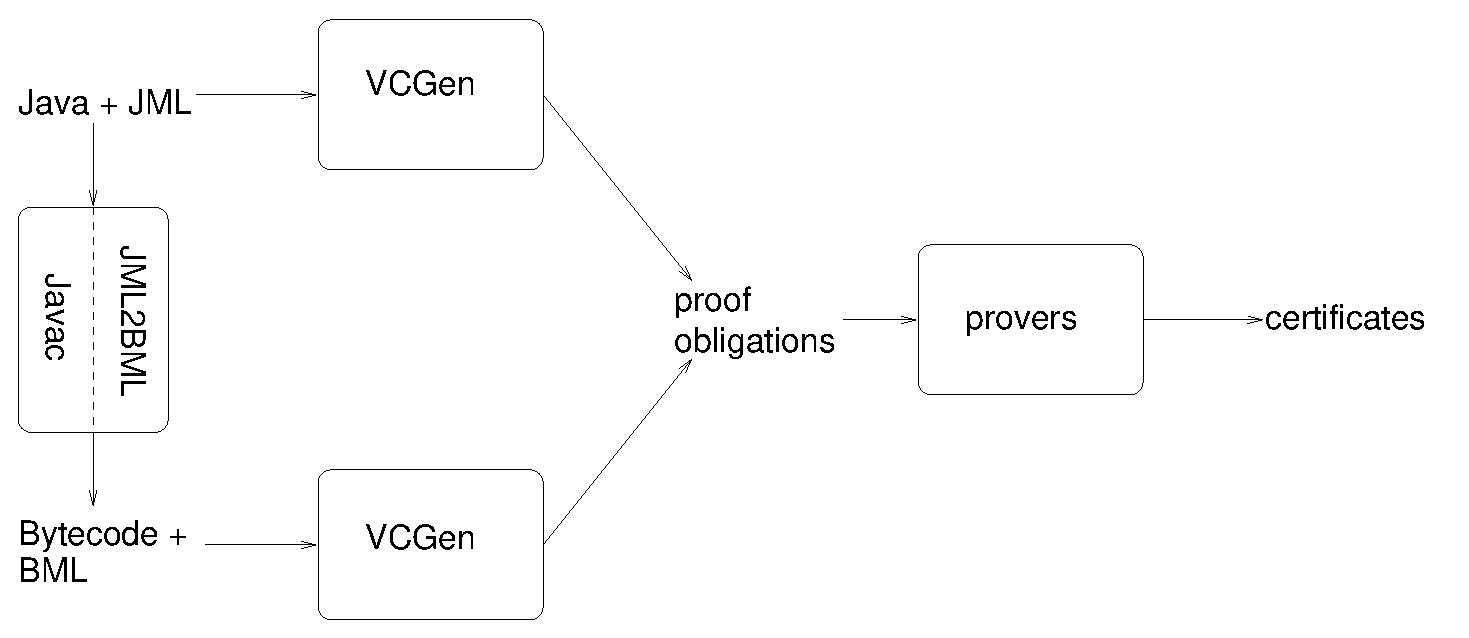
\includegraphics[width=0.8\textwidth]{toolset.eps} 
\vspace*{-1em}
\caption{Overview of \mobius tool set}\label{FigToolSet}
\end{center}
\end{figure}
\paragraph{Tool support}
As part of the \mobius project, we plan to develop a program
verification tool set that supports both JML and
BML. Figure~\ref{FigToolSet} outlines the general architecture of this
tool set. Thus, both Java/JML and bytecode/BML can be used as input
application. Annotated programs are translated into a guarded
command format, for which an appropriate verification condition
generator is used to generate proof obligations that can be discharged
with a theorem prover (either automatic or interactive). To support
the PCC platform, the provers will be instrumented to produce
certificates. In addition, source code applications annotated with JML
can be compiled into bytecode annotated with BML.

The development of the JML subcomponent of the tool set will be based
on experiences with ESC/Java~\cite{CokK04} and JACK~\cite{BurdyRL03}.
Several tools and algorithms (notably the compiler and the
verification condition generator) for BML have already been
implemented, see~\cite{BP06JSV,Pavlova:phd}, but more work is needed
to cover the whole language. Moreover, to make the tool set usable in
practice, we will also need a tool to inspect and write BML
specifications directly, and a run-time checker for BML
specifications. The latter can be implemented by a code
transformation, inserting explicit run-time checks in the bytecode, or
by extending the virtual machine to take the user-specific attributes
with specifications into account.  It is also important to have tool
support for checking the structural and typing constraints for BML
specifications. Such a tool can be built as an extension the Java
bytecode verifier.

Our initial experiments with compilation of specifications has shown
that there exists indeed a correspondence between the proof
obligations generated at source and at bytecode level, modulo
differences in elimination of trivial goals, handling of boolean
expressions, and the naming convention of generated
variables~\cite{Pavlova:phd}. Moreover, when the proofs are done with
the Coq prover, different names are generated for hypotheses at source
code and bytecode level. It is future work to clean up the
compilation, so there is a one-to-one correspondence.




 

\paragraph{Related work}
The interest in specification and verification of bytecode
applications is quite recent, and not too much work has been done in
that direction. Several logics have been developed to reason about
bytecode, \emph{e.g.}~by Bannwart \& M\"uller~\cite{BannwartMueller05}
and within the MRG project~\cite{AspinallEtAl:TPHOLs2004}. However, in
this work the main focus was the development of a sound proof system,
while the focus of BML is to write understandable specifications for
bytecode. JVer is a tool to verify annotated
bytecode~\cite{ChanderEILN05}. However, as specification language they
use a subset of JML, \emph{i.e.}\ a source code level specification language.

The development of BML is clearly inspired by the development of the
JML specification language~\cite{JMLReferenceManual05}. Both JML and
BML follow the Design by Contract principle introduced first in
Eiffel~\cite{Meyer97}. The Boogie project~\cite{BarnettCDJL05}
introduces in similarly the Design by Contract principles into the C\#
programming language, both at source code level and for CIL, the .NET
intermediate language.  The possibility to check a property at
run-time, using the \texttt{assert} construct, has been long 
adopted in the C programming language and recently also in Java (Java
1.5, see \cite[\S 14.10]{JLS}). 

Finally, we should mention the Extended Virtual Platform
project\footnote{See
\url{http://www.cs.usm.maine.edu/~mroyer/xvp/}.}. This project aims at
developing a framework that allows to compile JML annotations, to
allow run-time checking~\cite{AlagicXVP05}. However, in contrast to
our work, they do not intend to do static verification of bytecode
programs. Moreover, their platform takes JML-annotated source code
files as starting point, so it is not possible to annotate bytecode
applications directly.

\vspace*{-.5em}
\subsubsection*{Acknowledgements}
We thank Lennart Beringer and Olha Shkaravska for discussions about
the semantics of BML. 
%\vspace*{-.5em}




\bibliographystyle{plain}
\bibliography{bytecode,../specification,/user/mhuisman/home/Research/Everest/Biblio/everest}

%\appendix
%% generated and manually adapted from BML-grammar.texinfo

\newdimen{\standardmargin}  \setlength{\standardmargin}{15pt}
\newdimen{\tableindent}     \setlength{\tableindent}{50pt}
\newbox\ItemBox

\setcounter{secnumdepth}{5}       
\setcounter{tocdepth}{5}          

\def\lqHook{\char16 }\def\rqHook{\char17 }\def\lnqHook{\char96 }\def\rnqHook{\char39 }%
%\usepackage{varioref}         




\newcommand{\lbr}{\ifvmode\else\unskip\relax\nobreak\hfil\break\fi}




\newenvironment{display}[1][\standardmargin]%
                       {\begingroup\def~{\mbox{ }}\let\\=\lbr
                        \list{}{\listparindent0pt  \itemindent0pt
                        \rightmargin0pt    \leftmargin#1}%
                \item}
               {\endlist\endgroup}



\renewenvironment{quote}
                 {\list{}{\leftmargin\standardmargin\rightmargin\leftmargin}%
                  \item\relax}
                 {\endlist}



\makeatletter
\newcommand\Nopagebreak{\let\if@nobreak\iftrue \nopagebreak}
\makeatother





\newcommand{\tabletermHook}[1]{#1}

\newcommand{\kbdHook}[1]{\mbox{\ttfamily\slshape #1}}

\newcommand{\keyHook}[1]{{\fboxsep2pt\fbox{\sffamily\footnotesize #1}}}
\newcommand{\sampHook}[1]{\lnqHook\texttt{#1}\rnqHook}
\newcommand{\verbHook}[1]{\mbox{\ttfamily #1}}
\newcommand{\envHook}[1]{\mbox{\ttfamily #1}}
\newcommand{\fileHook}[1]{\lnqHook\texttt{#1}\rnqHook}
\newcommand{\commandHook}[1]{\mbox{\ttfamily #1}}
\newcommand{\optionHook}[1]{\lnqHook\mbox{\ttfamily #1}\rnqHook}
\newcommand{\dfnHook}[1]{\emph{#1}}
\newcommand{\citeHook}[1]{\textit{#1}}
\newcommand{\abbrevwordHook}[1]{#1}
\newcommand{\abbrevdescHook}[1]{ (#1)}
\newcommand{\acronymwordHook}[1]{\mbox{#1}}
\newcommand{\acronymdescHook}[1]{\footnote{#1}}
\newcommand{\urlHook}[1]{#1}
\newcommand{\emailHook}[1]{#1}

\newcommand{\emphHook}[1]{\emph{#1}}
\newcommand{\strongHook}[1]{\textbf{#1}}
\newcommand{\scHook}[1]{\textsc{#1}}
\newcommand{\slantedHook}[1]{\textsl{#1}}
\newcommand{\sansserifHook}[1]{\textsf{#1}}
\newcommand{\iHook}[1]{\textit{#1}}
\newcommand{\bHook}[1]{\textbf{#1}}
\newcommand{\tHook}[1]{\texttt{#1}}
\newcommand{\rHook}[1]{\textrm{#1}}
\newcommand{\dmnHook}[1]{\,\mbox{#1}}
\newcommand{\mathHook}[1]{\ensuremath{#1}}
\newcommand{\footnoteHook}[1]{\footnote{#1}}



\newenvironment{quotationHook}{\begin{quote}}{\end{quote}}
\newenvironment{copyingHook}{\begin{quote}}{\end{quote}}
\newenvironment{verbatimHook}{\begin{display}[0pt]\ttfamily}{\end{display}}
\newenvironment{exampleHook}{\begin{display}\ttfamily}{\end{display}}
\newenvironment{lispHook}{\begin{display}\ttfamily}{\end{display}}
\newenvironment{displayHook}{\begin{display}\relax}{\end{display}}
\newenvironment{formatHook}{\begin{display}[0pt]}{\end{display}}

\newenvironment{smallexampleHook}{\begin{small}\begin{exampleHook}}%
    {\end{exampleHook}\end{small}}
\newenvironment{smalldisplayHook}{\begin{small}\begin{displayHook}}%
    {\end{displayHook}\end{small}}
\newenvironment{smallformatHook}{\begin{small}\begin{formatHook}}%
    {\end{formatHook}\end{small}}
\newenvironment{smalllispHook}{\begin{small}\begin{lispHook}}%
    {\end{lispHook}\end{small}}

\newenvironment{flushleftHook}{\begin{flushleft}}{\end{flushleft}}
\newenvironment{flushrightHook}{\begin{flushright}}{\end{flushright}}
\newenvironment{groupHook}{\begin{samepage}}{\end{samepage}}

\newenvironment{cartoucheHook}{\begin{center}\shadowbox\bgroup
    \hbox to \hsize\bgroup\begin{minipage}{\hsize}}%
    {\end{minipage}\hss\egroup\egroup\end{center}}

\newcommand{\centerHook}[1]{\centerline{#1}}




\newenvironment{definitionitem}[1][\standardmargin]
               {\list{}{\listparindent0pt  \itemindent0pt
                        \rightmargin0pt    \leftmargin#1}%
                \item\removelastskip\relax}
               {\endlist}

\sloppy               
\hbadness20000





%\PassOptionsToPackage{hyphens}{url}
%\newcommand{\xhyphen}{\discretionary{\char127}{}{-}}
%\IfFileExists{pdfcprot.sty}{\usepackage[activate]{pdfcprot}}{}
%\usepackage[%
%  pagebackref=true,pdfstartview=FitH,
%  pdfcreator={texi2latex + LaTeX with hyperref package},
%  pdfpagelayout=OneColumn,
%  bookmarks=true,bookmarksopen=false,  colorlinks,pdfpagelabels=true,
%  draft=false,breaklinks=true,plainpages=false]{hyperref}[2000/05/08]  \hypersetup{%
%    pdftitle={BML grammar},
%    pdfsubject={<setfilename>BML-grammar.texinfo</setfilename>},
%    pdfauthor={}
%  }
%\urlstyle{rm}




%\usepackage{hypbmsec}



%\InputIfFileExists{texi2latex.cfg}%
%  {\message{Loading global configuration file texi2latex.cfg}}{}
%\InputIfFileExists{\jobname-t2l.cfg}%
%  {\message{Loading local configuration file \jobname-t2l.cfg}}{}



%\begin{document}


\gdef\InsertLabelMaybe{\label{predicates-and-specification-expressions}\gdef\InsertLabelMaybe{}}
\section{Grammar for BML predicates and specification expressions}\label{AppBML}\InsertLabelMaybe

\textbf{NOTE: We intend to set up a webpage with the complete BML grammar 
before publication. This grammar is included for the reviewer's
convenience, but will not be included in the final version of the
paper.}

As in the JML Reference Manual~\cite{JMLReferenceManual05}, we use an
extended Backus-Nauer Form (BNF) grammar to describe the syntax of
JML. The extensions are as follows~\cite{Ledgard80}.

\begin{itemize}
\item Nonterminal symbols are written as follows: \varHook{nonterminal}.

\item Terminal symbols are written as follows: \codeHook{terminal}.

\item Square brackets ([ and ]) surround optional text. Notice that
\codeHook{[} and \codeHook{]} are terminal symbols.  

\item The notation \dots\ means that the preceding nonterminal or group of optional text can be repeated zero or more times.  
\end{itemize}

\begin{displayHook}\\\relax {\varHook{predicate}}~::=~{\varHook{spec-{}expression}}\\\relax {\varHook{spec-{}expression-{}list}}~::=~{\varHook{spec-{}expression}}\\\relax ~~~~~~~~~~~~~~~~~~~~~~~~~[~{\codeHook{,}}~{\varHook{spec-{}expression}}~]~\dots \@{}\\\relax {\varHook{spec-{}expression}}~::=~{\varHook{expression}}\\\relax {\varHook{expression-{}list}}~::=~{\varHook{expression}}~[~{\codeHook{,}}~{\varHook{expression}}~]~\dots \@{}\\\relax {\varHook{expression}}~::=~{\varHook{conditional-{}expr}}~\\\relax {\varHook{conditional-{}expr}}~::=~{\varHook{equivalence-{}expr}}\\\relax ~~~~~~~~~~~~~~~~~~~[~{\codeHook{?{}}}~{\varHook{conditional-{}expr}}~{\codeHook{:}}~{\varHook{conditional-{}expr}}~]\\\relax {\varHook{equivalence-{}expr}}~::=~{\varHook{implies-{}expr}}\\\relax ~~~~~~~~~~~~~~~~~~~~~[~{\varHook{equivalence-{}op}}~{\varHook{implies-{}expr}}~]~\dots \@{}\\\relax {\varHook{equivalence-{}op}}~::=~{\codeHook{<{}==>{}}}~{\mbox{\char124{}}}~{\codeHook{<{}=!{}=>{}}}\\\relax {\varHook{implies-{}expr}}~::=~{\varHook{logical-{}or-{}expr}}\\\relax ~~~~~~~~~~~~~[~{\codeHook{==>{}}}~{\varHook{implies-{}non-{}backward-{}expr}}~]\\\relax ~~~~~~~~{\mbox{\char124{}}}~{\varHook{logical-{}or-{}expr}}~{\codeHook{<{}==}}~{\varHook{logical-{}or-{}expr}}\\\relax ~~~~~~~~~~~~~[~{\codeHook{<{}==}}~{\varHook{logical-{}or-{}expr}}~]~\dots \@{}\\\relax {\varHook{implies-{}non-{}backward-{}expr}}~::=~{\varHook{logical-{}or-{}expr}}\\\relax ~~~~~~~~~~~~~[~{\codeHook{==>{}}}~{\varHook{implies-{}non-{}backward-{}expr}}~]\\\relax {\varHook{logical-{}or-{}expr}}~::=~{\varHook{logical-{}and-{}expr}}~[~`{}{\codeHook{{\mbox{\char124{}}}{\mbox{\char124{}}}}}'{}~{\varHook{logical-{}and-{}expr}}~]~\dots \@{}\\\relax {\varHook{logical-{}and-{}expr}}~::=~{\varHook{inclusive-{}or-{}expr}}~[~{\codeHook{\&\&}}~{\varHook{inclusive-{}or-{}expr}}~]~\dots \@{}\\\relax {\varHook{inclusive-{}or-{}expr}}~::=~{\varHook{exclusive-{}or-{}expr}}~[~`{}{\codeHook{{\mbox{\char124{}}}}}'{}~{\varHook{exclusive-{}or-{}expr}}~]~\dots \@{}\\\relax {\varHook{exclusive-{}or-{}expr}}~::=~{\varHook{and-{}expr}}~[~{\codeHook{{\mbox{\char94{}}}}}~{\varHook{and-{}expr}}~]~\dots \@{}\\\relax {\varHook{and-{}expr}}~::=~{\varHook{equality-{}expr}}~[~{\codeHook{\&}}~{\varHook{equality-{}expr}}~]~\dots \@{}\\\relax {\varHook{equality-{}expr}}~::=~{\varHook{relational-{}expr}}~[~{\codeHook{==}}~{\varHook{relational-{}expr}}]~\dots \@{}\\\relax ~~~~~~~~{\mbox{\char124{}}}~{\varHook{relational-{}expr}}~[~{\codeHook{!{}=}}~{\varHook{relational-{}expr}}]~\dots \@{}\\\relax {\varHook{relational-{}expr}}~::=~{\varHook{shift-{}expr}}~{\codeHook{<{}}}~{\varHook{shift-{}expr}}\\\relax ~~~~~~~~{\mbox{\char124{}}}~{\varHook{shift-{}expr}}~{\codeHook{>{}}}~{\varHook{shift-{}expr}}\\\relax ~~~~~~~~{\mbox{\char124{}}}~{\varHook{shift-{}expr}}~{\codeHook{<{}=}}~{\varHook{shift-{}expr}}\\\relax ~~~~~~~~{\mbox{\char124{}}}~{\varHook{shift-{}expr}}~{\codeHook{>{}=}}~{\varHook{shift-{}expr}}\\\relax ~~~~~~~~{\mbox{\char124{}}}~{\varHook{shift-{}expr}}~{\codeHook{<{}:}}~{\varHook{shift-{}expr}}\\\relax ~~~~~~~~{\mbox{\char124{}}}~{\varHook{shift-{}expr}}~[~{\codeHook{instanceof}}~{\varHook{type-{}spec}}~]\\\relax {\varHook{shift-{}expr}}~::=~{\varHook{additive-{}expr}}~[~{\varHook{shift-{}op}}~{\varHook{additive-{}expr}}~]~\dots \@{}\\\relax {\varHook{shift-{}op}}~::=~{\codeHook{<{}<{}}}~{\mbox{\char124{}}}~{\codeHook{>{}>{}}}~{\mbox{\char124{}}}~{\codeHook{>{}>{}>{}}}\\\relax {\varHook{additive-{}expr}}~::=~{\varHook{mult-{}expr}}~[~{\varHook{additive-{}op}}~{\varHook{mult-{}expr}}~]~\dots \@{}\\\relax {\varHook{additive-{}op}}~::=~{\codeHook{+}}~{\mbox{\char124{}}}~{\codeHook{-{}}}\\\relax {\varHook{mult-{}expr}}~::=~{\varHook{unary-{}expr}}~[~{\varHook{mult-{}op}}~{\varHook{unary-{}expr}}~]~\dots \@{}\\\relax {\varHook{mult-{}op}}~::=~{\codeHook{*}}~{\mbox{\char124{}}}~{\codeHook{/}}~{\mbox{\char124{}}}~{\codeHook{\%}}\\\relax {\varHook{unary-{}expr}}~::=~{\codeHook{(}}~{\varHook{type-{}spec}}~{\codeHook{)}}~{\varHook{unary-{}expr}}\\\relax ~~~~~~~~{\mbox{\char124{}}}~{\codeHook{+}}~{\varHook{unary-{}expr}}\\\relax ~~~~~~~~{\mbox{\char124{}}}~{\codeHook{-{}}}~{\varHook{unary-{}expr}}\\\relax ~~~~~~~~{\mbox{\char124{}}}~{\varHook{unary-{}expr-{}not-{}plus-{}minus}}\\\relax {\varHook{unary-{}expr-{}not-{}plus-{}minus}}~::=~{\codeHook{{\mbox{\char126{}}}}}~{\varHook{unary-{}expr}}\\\relax ~~~~~~~~{\mbox{\char124{}}}~{\codeHook{!{}}}~{\varHook{unary-{}expr}}\\\relax ~~~~~~~~{\mbox{\char124{}}}~{\codeHook{(}}~{\varHook{built-{}in-{}type}}~{\codeHook{)}}~{\varHook{unary-{}expr}}\\\relax ~~~~~~~~{\mbox{\char124{}}}~{\codeHook{(}}~{\varHook{reference-{}type}}~{\codeHook{)}}~{\varHook{unary-{}expr-{}not-{}plus-{}minus}}\\\relax ~~~~~~~~{\mbox{\char124{}}}~{\varHook{primary-{}expr}}~[~{\varHook{primary-{}suffix}}~]~\dots \@{}\\\relax {\varHook{primary-{}suffix}}~::=~{\codeHook{(}}~[~{\varHook{expression-{}list}}~]~{\codeHook{)}}\\\relax ~~~~~~~~{\mbox{\char124{}}}~`{}{\codeHook{[}}'{}~{\varHook{expression}}~`{}{\codeHook{]}}'{}\\\relax {\varHook{primary-{}expr}}~::=~~{\codeHook{{\mbox{\char92{}}}{\mbox{\char35{}}}}}{\varHook{natural}}~{\mbox{\char124{}}}~{\codeHook{lv[}}~{\varHook{natural}}~{\codeHook{]}}\\\relax ~~~~~~~~{\mbox{\char124{}}}~{\varHook{constant}}~{\mbox{\char124{}}}~{\codeHook{super}}~{\mbox{\char124{}}}~{\codeHook{true}}\\\relax ~~~~~~~~{\mbox{\char124{}}}~{\codeHook{false}}~{\mbox{\char124{}}}~{\codeHook{this}}~{\mbox{\char124{}}}~{\codeHook{null}}\\\relax ~~~~~~~~{\mbox{\char124{}}}~{\codeHook{(}}~{\varHook{expression}}~{\codeHook{)}}\\\relax ~~~~~~~~{\mbox{\char124{}}}~{\varHook{bml-{}primary}}\\\relax ~~~~~~~~{\mbox{\char124{}}}~{\varHook{jml-{}primary}}\\\relax {\varHook{built-{}in-{}type}}~::=~{\codeHook{void}}~{\mbox{\char124{}}}~{\codeHook{boolean}}~{\mbox{\char124{}}}~{\codeHook{byte}}\\\relax ~~~~~~~~{\mbox{\char124{}}}~{\codeHook{char}}~{\mbox{\char124{}}}~{\codeHook{short}}~{\mbox{\char124{}}}~{\codeHook{int}}\\\relax ~~~~~~~~{\mbox{\char124{}}}~{\codeHook{long}}~{\mbox{\char124{}}}~{\codeHook{float}}~{\mbox{\char124{}}}~{\codeHook{double}}\\\relax {\varHook{constant}}~::=~{\varHook{java-{}literal}}\\\relax {\varHook{bml-{}primary}}~::=~{\varHook{array-{}length-{}expression}}~{\mbox{\char124{}}}\\\relax ~~~~~~~~~~~{\mbox{\char124{}}}~{\varHook{opstack-{}counter-{}expression}}\\\relax ~~~~~~~~~~~{\mbox{\char124{}}}~{\varHook{stack-{}expresion}}\\\relax {\varHook{array-{}length-{}expression}}~::=~{\codeHook{length(}}~{\varHook{expression}}~{\codeHook{)}}\\\relax {\varHook{opstack-{}counter-{}expression}}~::=~{\codeHook{cntr}}\\\relax {\varHook{stack-{}expression}}~::=~{\codeHook{st(}}~{\varHook{additive-{}expr}}~{\codeHook{)}}\\\relax {\varHook{jml-{}primary}}~::=~{\varHook{result-{}expression}}\\\relax ~~~~~~~~{\mbox{\char124{}}}~{\varHook{old-{}expression}}\\\relax ~~~~~~~~{\mbox{\char124{}}}~{\varHook{fresh-{}expression}}\\\relax ~~~~~~~~{\mbox{\char124{}}}~{\varHook{nonnullelements-{}expression}}\\\relax ~~~~~~~~{\mbox{\char124{}}}~{\varHook{typeof-{}expression}}\\\relax ~~~~~~~~{\mbox{\char124{}}}~{\varHook{elemtype-{}expression}}\\\relax ~~~~~~~~{\mbox{\char124{}}}~{\varHook{type-{}expression}}\\\relax ~~~~~~~~{\mbox{\char124{}}}~{\varHook{spec-{}quantified-{}expr}}\\\relax {\varHook{result-{}expression}}~::=~{\codeHook{{\mbox{\char92{}}}result}}\\\relax {\varHook{old-{}expression}}~::=~{\codeHook{{\mbox{\char92{}}}old}}~{\codeHook{(}}~{\varHook{spec-{}expression}}~{\codeHook{)}}\\\relax ~~~~~~~~{\mbox{\char124{}}}~{\codeHook{{\mbox{\char92{}}}pre}}~{\codeHook{(}}~{\varHook{spec-{}expression}}~{\codeHook{)}}\\\relax {\varHook{fresh-{}expression}}~::=~{\codeHook{{\mbox{\char92{}}}fresh}}~{\codeHook{(}}~{\varHook{spec-{}expression-{}list}}~{\codeHook{)}}\\\relax {\varHook{nonnullelements-{}expression}}~::=~{\codeHook{{\mbox{\char92{}}}nonnullelements}}~{\codeHook{(}}~{\varHook{spec-{}expression}}~{\codeHook{)}}\\\relax {\varHook{typeof-{}expression}}~::=~{\codeHook{{\mbox{\char92{}}}typeof}}~{\codeHook{(}}~{\varHook{spec-{}expression}}~{\codeHook{)}}\\\relax {\varHook{elemtype-{}expression}}~::=~{\codeHook{{\mbox{\char92{}}}elemtype}}~{\codeHook{(}}~{\varHook{spec-{}expression}}~{\codeHook{)}}\\\relax {\varHook{type-{}expression}}~::=~{\codeHook{{\mbox{\char92{}}}type}}~{\codeHook{(}}~{\varHook{type}}~{\codeHook{)}}\\\relax {\varHook{spec-{}quantified-{}expr}}~::=~{\codeHook{(}}~{\varHook{quantifier}}~{\varHook{quantified-{}var-{}decls}}~{\codeHook{;}}\\\relax ~~~~~~~~~~~~~~~~~~~~~~~~~~~[~[~{\varHook{predicate}}~]~{\codeHook{;}}~]\\\relax ~~~~~~~~~~~~~~~~~~~~~~~~~~~{\varHook{spec-{}expression}}~{\codeHook{)}}\\\relax {\varHook{quantifier}}~::=~{\codeHook{{\mbox{\char92{}}}forall}}~{\mbox{\char124{}}}~{\codeHook{{\mbox{\char92{}}}exists}}\\\relax {\varHook{quantified-{}var-{}decls}}~::=~[~{\varHook{bound-{}var-{}modifiers}}~]~{\varHook{type-{}spec}}~{\varHook{quantified-{}var-{}declarator}}\\\relax ~~~~~~~~~~~~~~~~~~~~~~~~~[~{\codeHook{,}}~{\varHook{quantified-{}var-{}declarator}}~]~\dots \@{}\\\relax {\varHook{quantified-{}var-{}declarator}}~::=~{\varHook{ident}}~[~{\varHook{dims}}~]\\\relax {\varHook{bound-{}var-{}modifiers}}~::=~{\codeHook{non{\mbox{\char95{}}}null}}~{\mbox{\char124{}}}~{\codeHook{nullable}}\\\relax {\varHook{store-{}ref-{}list}}~::=~{\varHook{store-{}ref}}~[~{\codeHook{,}}~{\varHook{store-{}ref}}~]~\dots \@{}\\\relax {\varHook{store-{}ref}}~::=~{\varHook{store-{}ref-{}expression}}\\\relax ~~~~~~~~{\mbox{\char124{}}}~{\varHook{store-{}ref-{}keyword}}\\\relax {\varHook{store-{}ref-{}expression}}~::=~{\varHook{store-{}ref-{}name}}~[~{\varHook{store-{}ref-{}name-{}suffix}}~]~\dots \@{}\\\relax {\varHook{store-{}ref-{}name}}~::=~{\codeHook{{\mbox{\char92{}}}{\mbox{\char35{}}}}}~{\varHook{natural}}~{\mbox{\char124{}}}~{\codeHook{super}}~{\mbox{\char124{}}}~{\codeHook{this}}\\\relax {\varHook{store-{}ref-{}name-{}suffix}}~::=~{\codeHook{(}}~{\varHook{store-{}ref-{}expression}}~{\codeHook{)}}\\\relax ~~~~~~~~{\mbox{\char124{}}}~`{}{\codeHook{[}}'{}~{\varHook{spec-{}array-{}ref-{}expr}}~`{}{\codeHook{]}}'{}\\\relax {\varHook{spec-{}array-{}ref-{}expr}}~::=~{\varHook{spec-{}expression}}\\\relax ~~~~~~~~{\mbox{\char124{}}}~{\varHook{spec-{}expression}}~{\codeHook{..}}~{\varHook{spec-{}expression}}\\\relax ~~~~~~~~{\mbox{\char124{}}}~{\codeHook{*}}\\\relax {\varHook{store-{}ref-{}keyword}}~::=~{\codeHook{{\mbox{\char92{}}}nothing}}~{\mbox{\char124{}}}~{\codeHook{{\mbox{\char92{}}}everything}}~{\mbox{\char124{}}}~{\codeHook{{\mbox{\char92{}}}not{\mbox{\char95{}}}specified}}\end{displayHook}


\end{document}
